% ============================================================================
%  VSEPR_SIM_INDEX.tex — Standalone Reading Guide and Quick Reference
%  Lighter document (~15 pages) with all overview figures, no PDF includes.
%  Compile:  pdflatex VSEPR_SIM_INDEX.tex  (run twice for refs)
% ============================================================================
\documentclass[11pt, letterpaper]{article}

\usepackage[top=0.9in, bottom=0.9in, left=1.0in, right=1.0in]{geometry}
\usepackage[T1]{fontenc}
\usepackage{lmodern}
\usepackage{microtype}
\usepackage{amsmath, amssymb}
\usepackage{booktabs}
\usepackage{longtable}
\usepackage{graphicx}
\usepackage{subcaption}
\usepackage{float}
\usepackage{xcolor}
\usepackage{enumitem}
\usepackage{multicol}
\usepackage{fancyhdr}
\usepackage[
  colorlinks=true, linkcolor={blue!60!black},
  urlcolor={purple!60!black}, bookmarks=true
]{hyperref}

\graphicspath{{figures/}}

\definecolor{darkblue}{RGB}{26,82,118}
\definecolor{darkgreen}{RGB}{30,130,76}
\definecolor{darkred}{RGB}{192,57,43}

\pagestyle{fancy}
\fancyhf{}
\fancyhead[L]{\small\textit{VSEPR-SIM Documentation Index}}
\fancyhead[R]{\small\textit{v3.0.0}}
\fancyfoot[C]{\thepage}

\setlist{nosep, leftmargin=1.5em}

\title{%
  \textbf{\color{darkblue}\Huge VSEPR-SIM}\\[4pt]
  {\Large } \\[6pt]
  {\large 43 Documents $\cdot$ 759 Pages $\cdot$ 96 Figures $\cdot$ 500+ Tests}
}
\author{VSEPR-SIM Project}
\date{Version 3.0.0 --- \today}

\begin{document}
\maketitle
\tableofcontents
\clearpage

% ════════════════════════════════════════════════════════════════════════════
\section{Platform Overview}
% ════════════════════════════════════════════════════════════════════════════

\textbf{VSEPR-SIM} is a research-oriented, deterministic, atomistic simulation
and analysis platform.  It bridges scientific theory, molecular identity,
deterministic structural generation, atomistic analysis, visualization,
and computational reporting.

\begin{figure}[H]
\centering
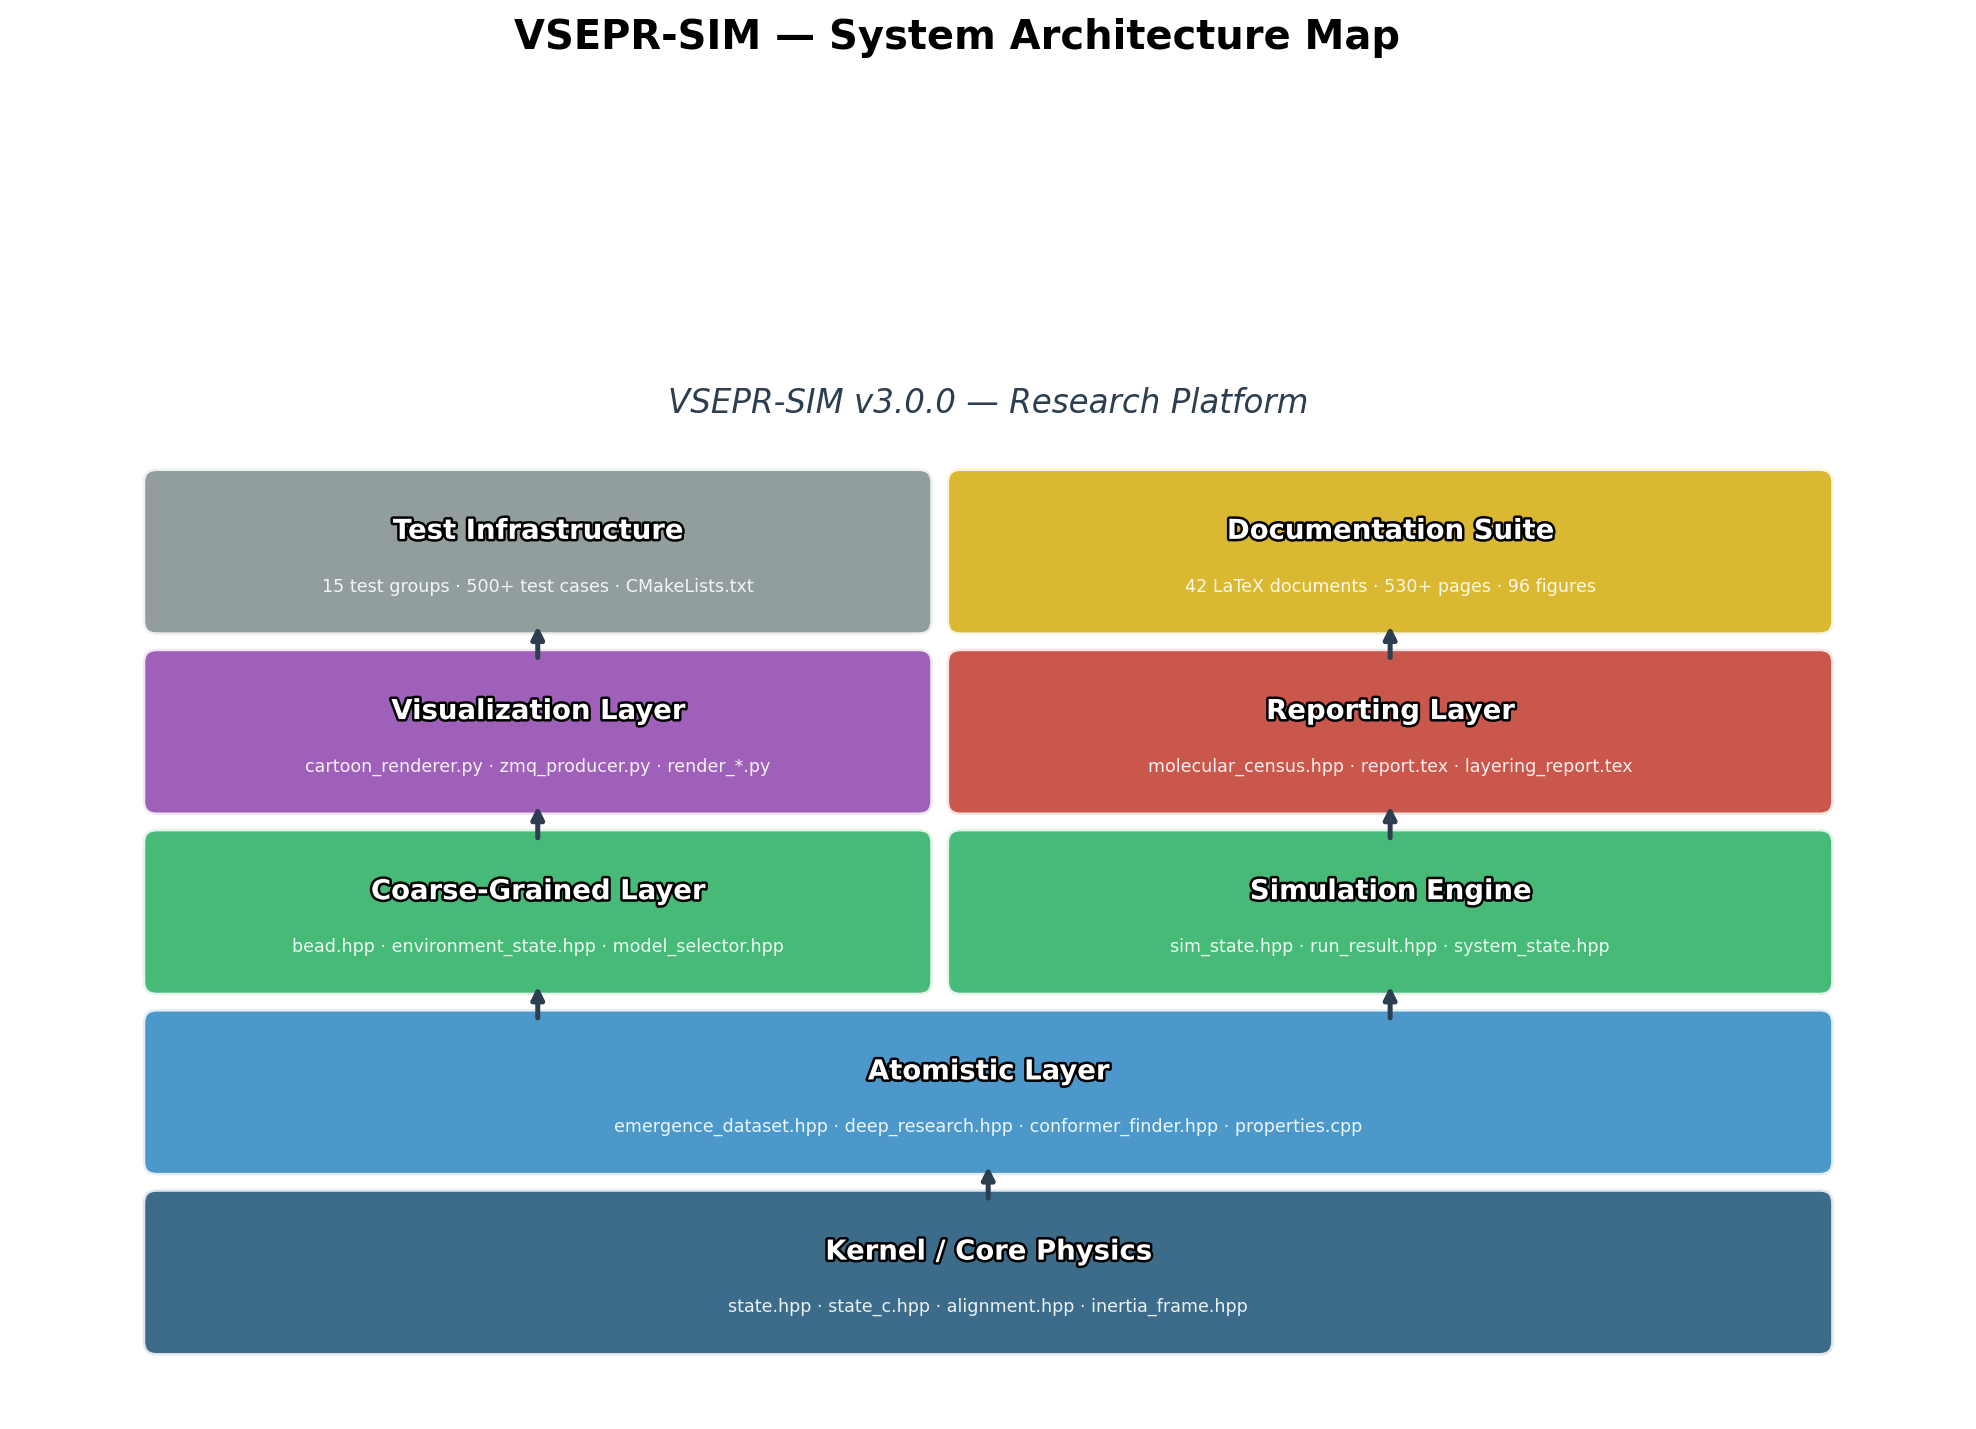
\includegraphics[width=0.95\textwidth]{overview_architecture_map.png}
\caption{System architecture map: eight layers from the physics kernel through documentation.}
\end{figure}

\subsection{Design Philosophy}
\begin{itemize}
\item \textbf{Deterministic} over theatrical---reproducible outputs, no hidden state.
\item \textbf{Anti-black-box}---every mapping, metric, and intermediate result is inspectable.
\item \textbf{Scientific coherence} over feature sprawl.
\item \textbf{Research utility} over interface vanity.
\end{itemize}

\subsection{Scientific Workflow}

\begin{figure}[H]
\centering
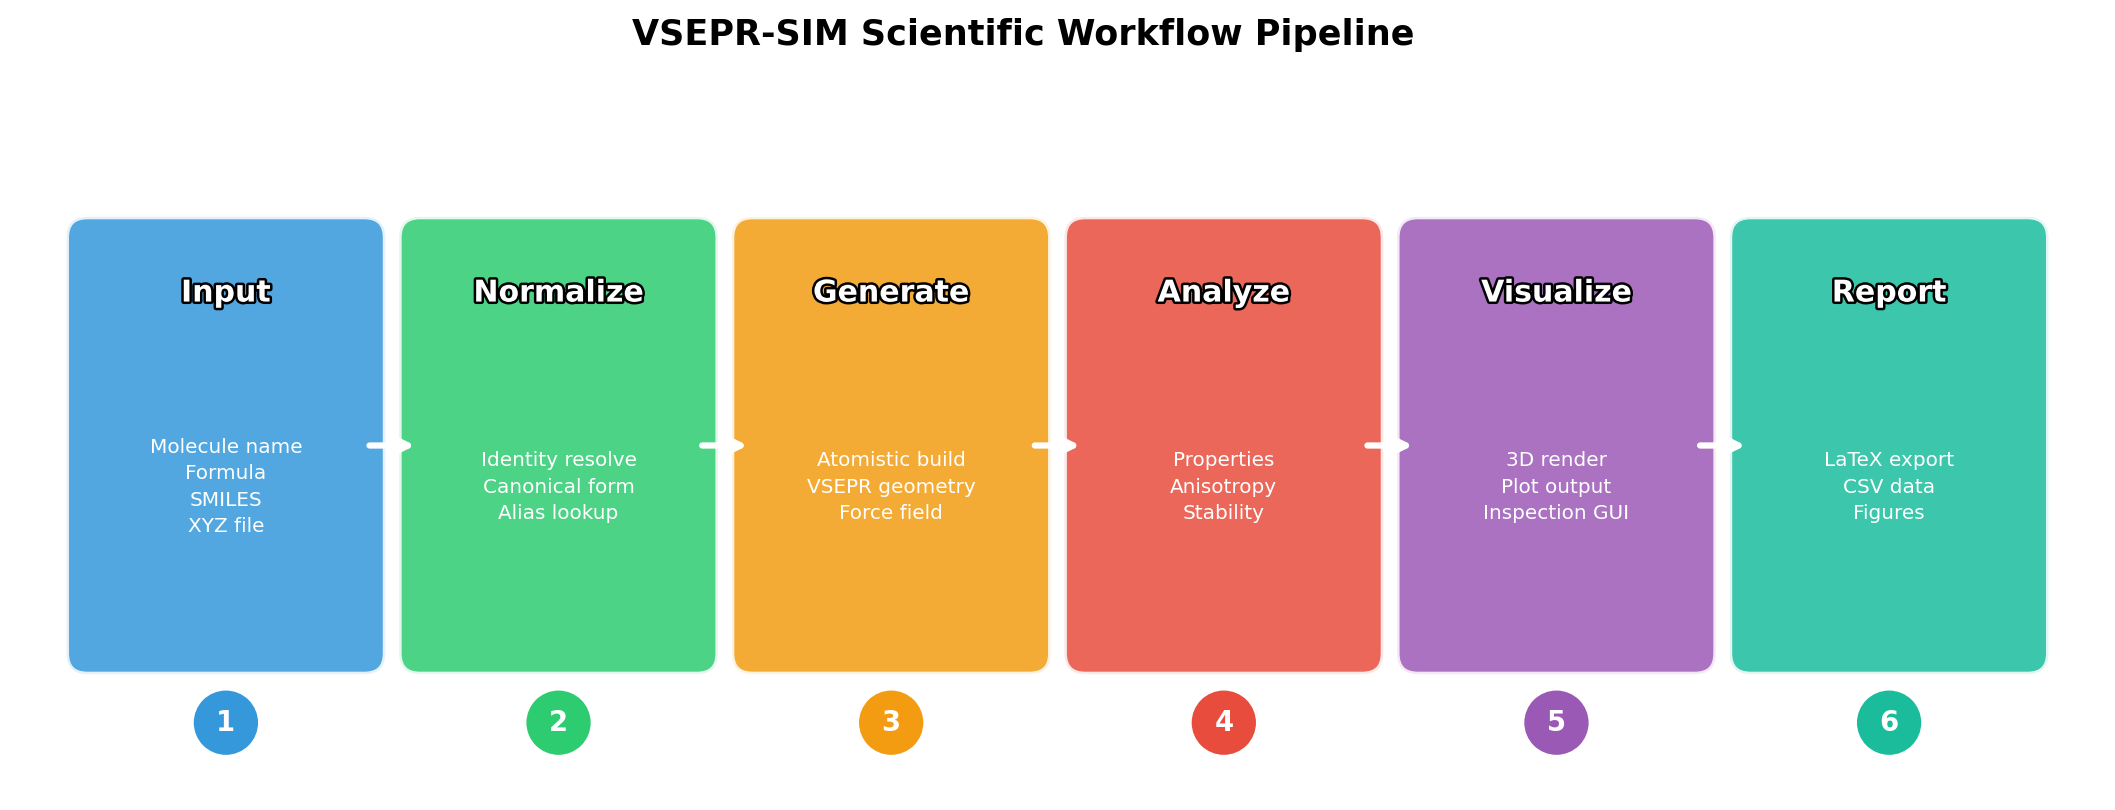
\includegraphics[width=0.95\textwidth]{overview_workflow_pipeline.png}
\caption{Six-stage pipeline: Input $\to$ Normalize $\to$ Generate $\to$ Analyze $\to$ Visualize $\to$ Report.}
\end{figure}


% ════════════════════════════════════════════════════════════════════════════
\section{Complete Document Inventory}
% ════════════════════════════════════════════════════════════════════════════

\begin{figure}[H]
\centering
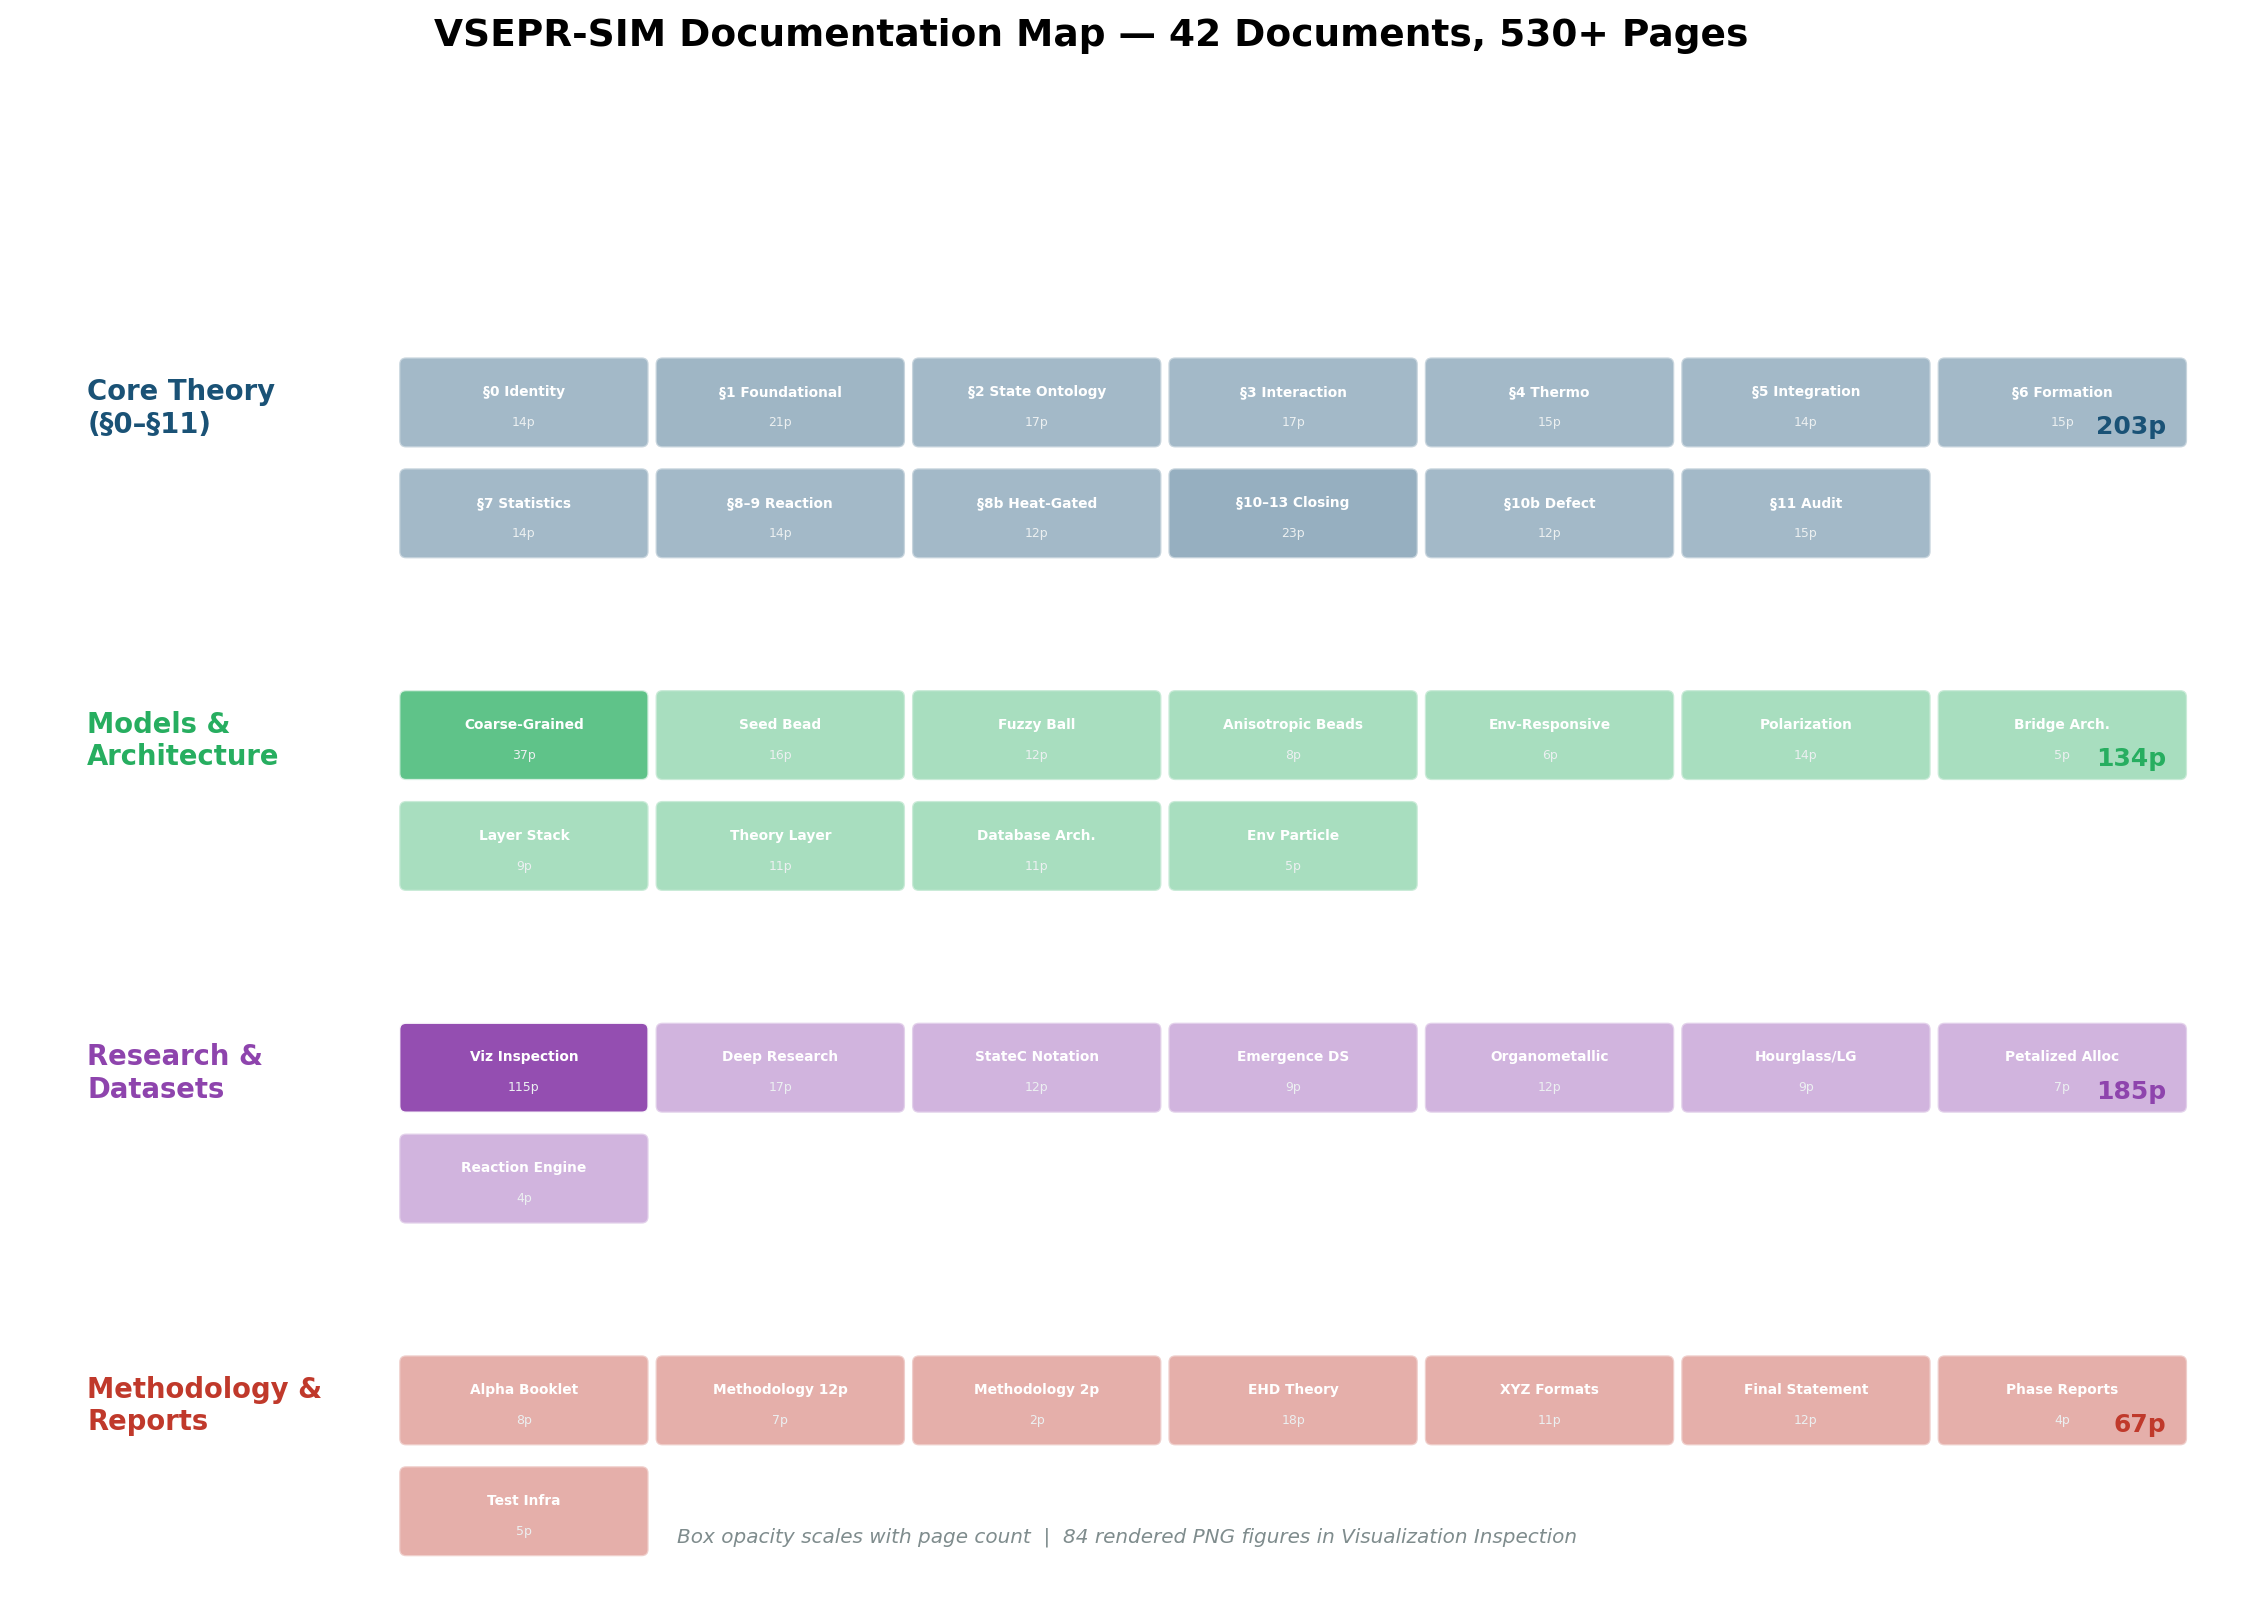
\includegraphics[width=0.95\textwidth]{overview_document_map.png}
\caption{Documentation map. Box opacity scales with page count.}
\end{figure}

\begin{figure}[H]
\centering
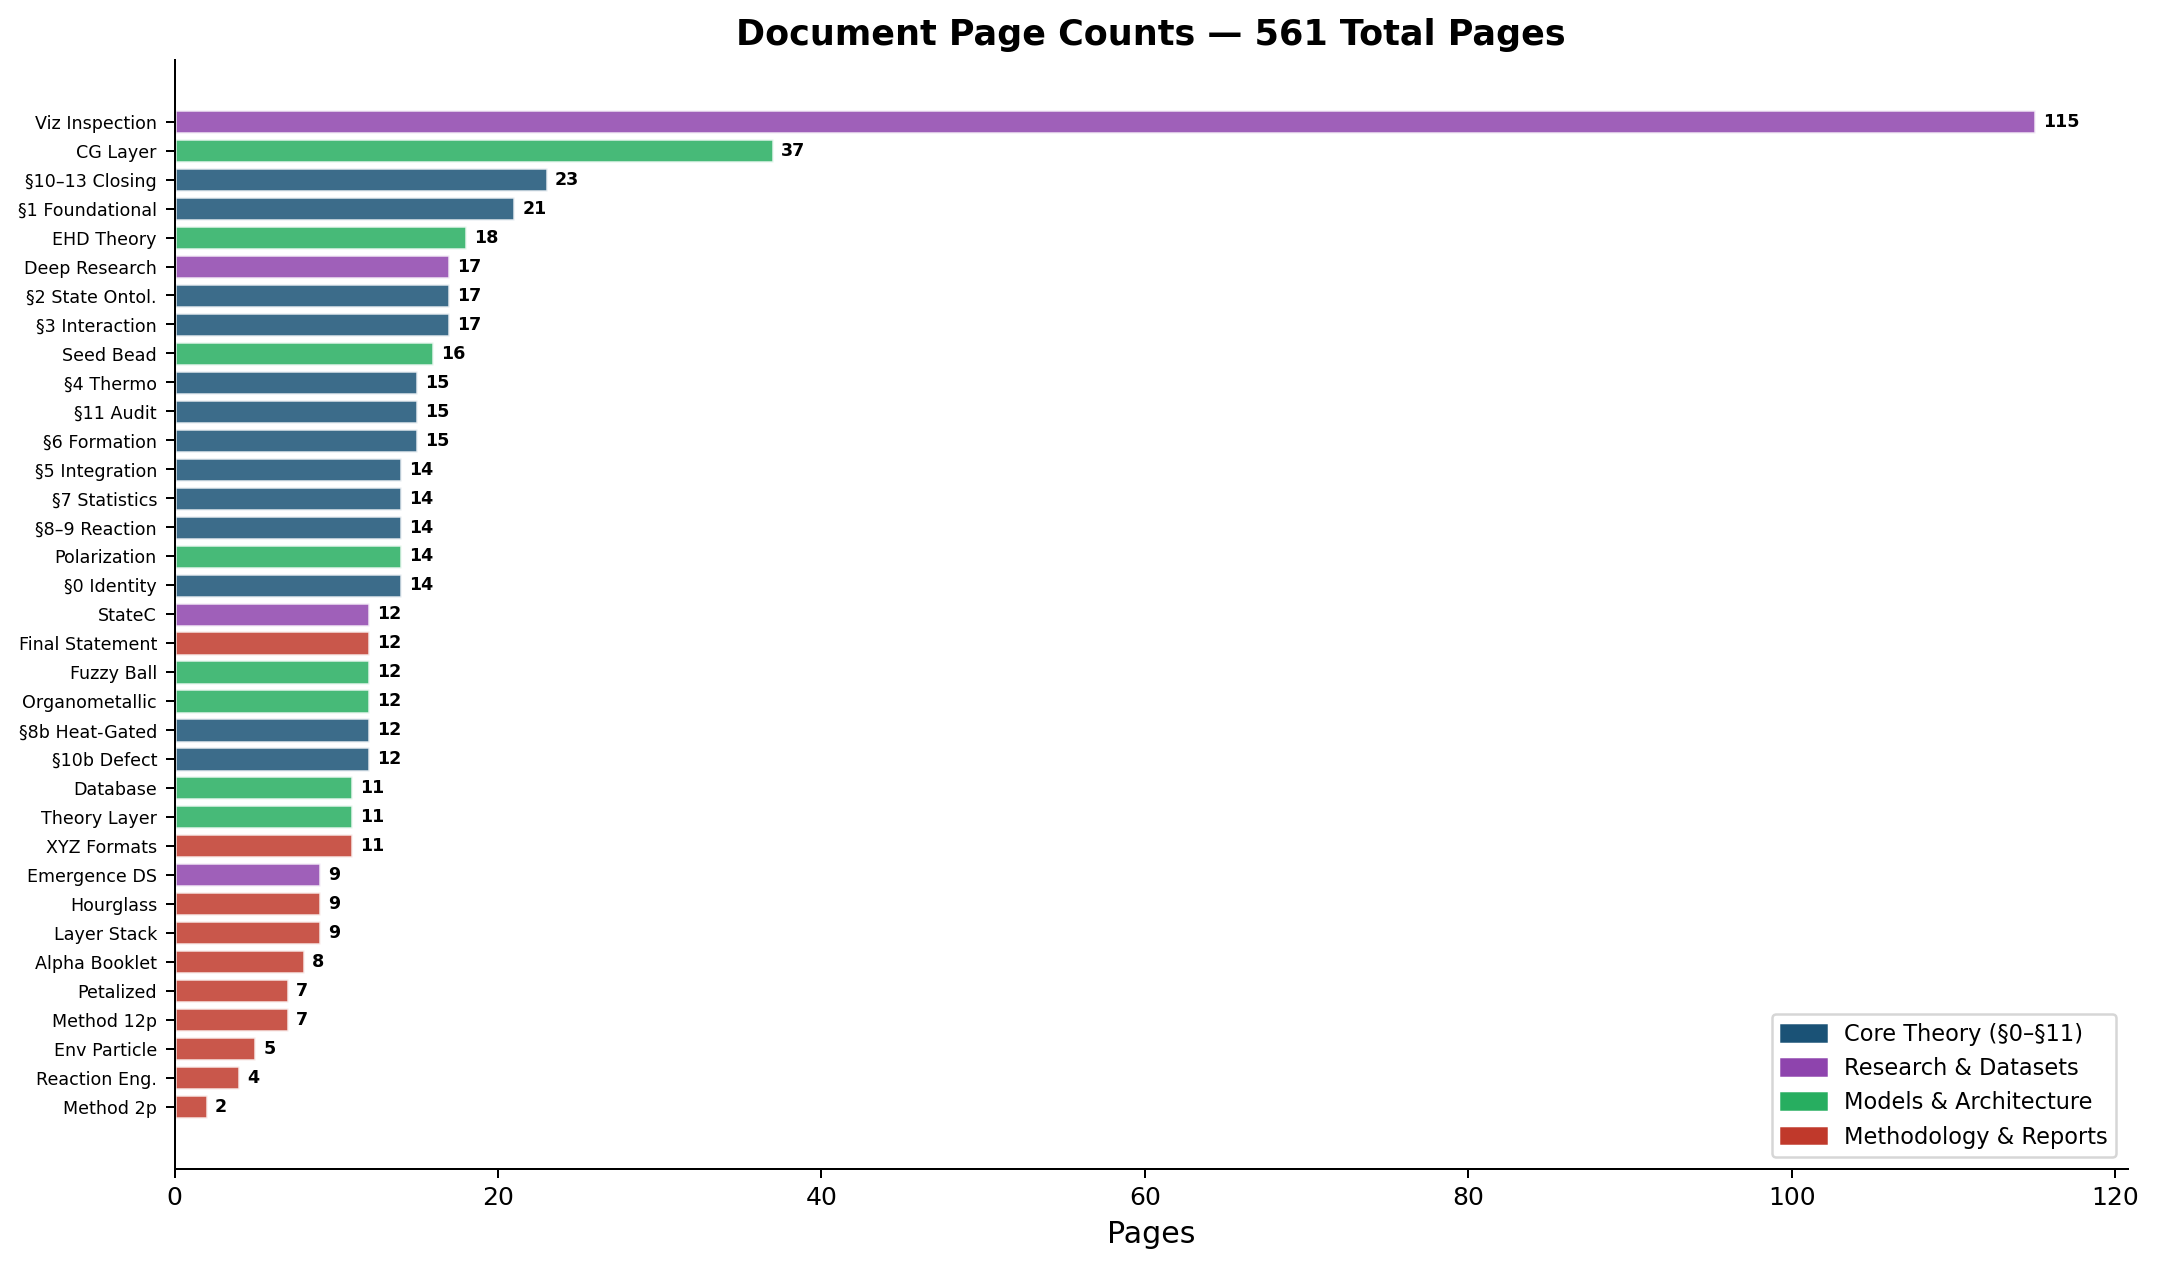
\includegraphics[width=0.95\textwidth]{overview_page_counts.png}
\caption{Page counts for all documents, colored by category.}
\end{figure}

\subsection{Part I: Core Theory ($\sim$203 pages)}

\begin{center}
\renewcommand{\arraystretch}{1.2}
\begin{tabular}{clrl}
\toprule
\textbf{\#} & \textbf{Document File} & \textbf{Pages} & \textbf{Key Topics} \\
\midrule
0  & \texttt{section0\_identity\_state\_decomposition}  & 14 & Identity/state split, $\mathcal{I}$/$\mathcal{S}$ \\
1  & \texttt{section1\_foundational\_thesis}            & 21 & Emergence boundary, scope \\
2  & \texttt{section2\_state\_ontology}                 & 17 & State definition, $S$ formal spec \\
3  & \texttt{section3\_interaction\_model}              & 17 & Force fields, potentials \\
4  & \texttt{section4\_thermodynamics}                  & 15 & Free energy, partition fn \\
5  & \texttt{section5\_integration}                     & 14 & Velocity Verlet, symplectic \\
6  & \texttt{section6\_formation\_physics}              & 15 & Nucleation, growth \\
7  & \texttt{section7\_statistical\_interpretation}     & 14 & Ensemble averages, ergodicity \\
8--9 & \texttt{section8\_9\_reaction\_electronic}       & 14 & Reaction paths, electronic \\
8b & \texttt{section8b\_heat\_gated\_reaction\_control} & 12 & Thermal activation barriers \\
10--13 & \texttt{section10\_12\_13\_closing}            & 23 & Extended discussion, outlook \\
10b & \texttt{section10b\_defect\_microstate\_classification} & 12 & Defect taxonomy \\
11 & \texttt{section11\_self\_audit}                    & 15 & Self-audit (100 tests+) \\
12 & \texttt{(in section10\_12\_13\_closing)}           & -- & Validation doctrine (100 tests+) \\
13 & \texttt{(in section10\_12\_13\_closing)}           & -- & Expansion layers (100 tests+) \\
14 & \texttt{(planned)}                                & -- & Atomistic engine (100 tests+) \\
15 & \texttt{(planned)}                                & -- & Formation, chemical, pipes (100 tests+) \\
\bottomrule
\end{tabular}
\end{center}

\subsection{Part II: Models and Architecture ($\sim$134 pages)}

\begin{center}
\renewcommand{\arraystretch}{1.2}
\begin{tabular}{lrl}
\toprule
\textbf{Document File} & \textbf{Pages} & \textbf{Key Topics} \\
\midrule
\texttt{section\_coarse\_grained\_layer}        & 37 & Bead mapping, CG force fields \\
\texttt{section\_seed\_bead\_model}             & 16 & Seed bead initialization \\
\texttt{section\_fuzzy\_ball\_model}            & 12 & Soft-core representation \\
\texttt{section\_anisotropic\_beads}            &  8 & Ellipsoidal beads, Gay-Berne \\
\texttt{section\_environment\_responsive\_beads} &  6 & Adaptive bead properties \\
\texttt{section\_polarization\_models}          & 14 & Alpha model, dipole response \\
\texttt{section\_bridge\_architecture}          &  5 & Multi-scale bridging \\
\texttt{section\_layer\_stack}                  &  9 & Layer organization \\
\texttt{section\_theory\_layer}                 & 11 & Theory abstraction interface \\
\texttt{section\_database\_architecture}        & 11 & Molecular database schema \\
\texttt{section\_env\_particle\_extension}      &  5 & Environment particles \\
\bottomrule
\end{tabular}
\end{center}

\begin{figure}[H]
\centering
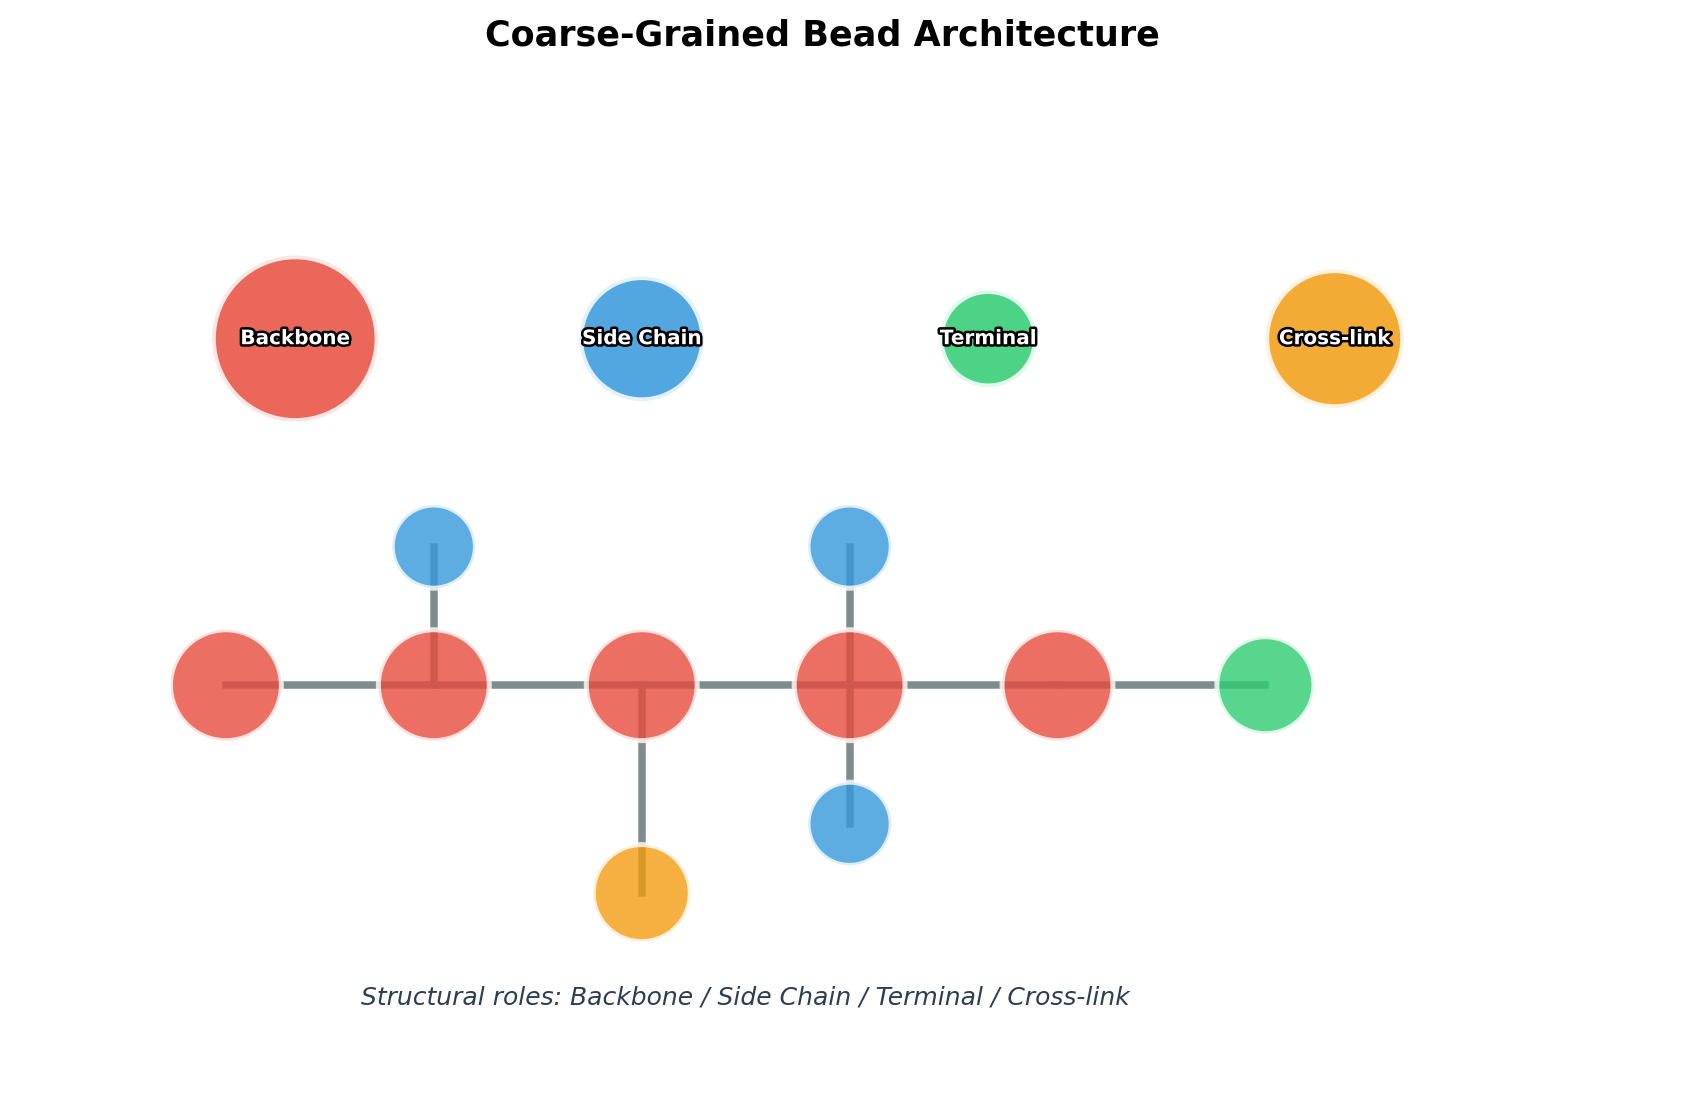
\includegraphics[width=0.85\textwidth]{overview_bead_types.png}
\caption{Bead structural roles: backbone, side chain, terminal, cross-link.}
\end{figure}

\begin{figure}[H]
\centering
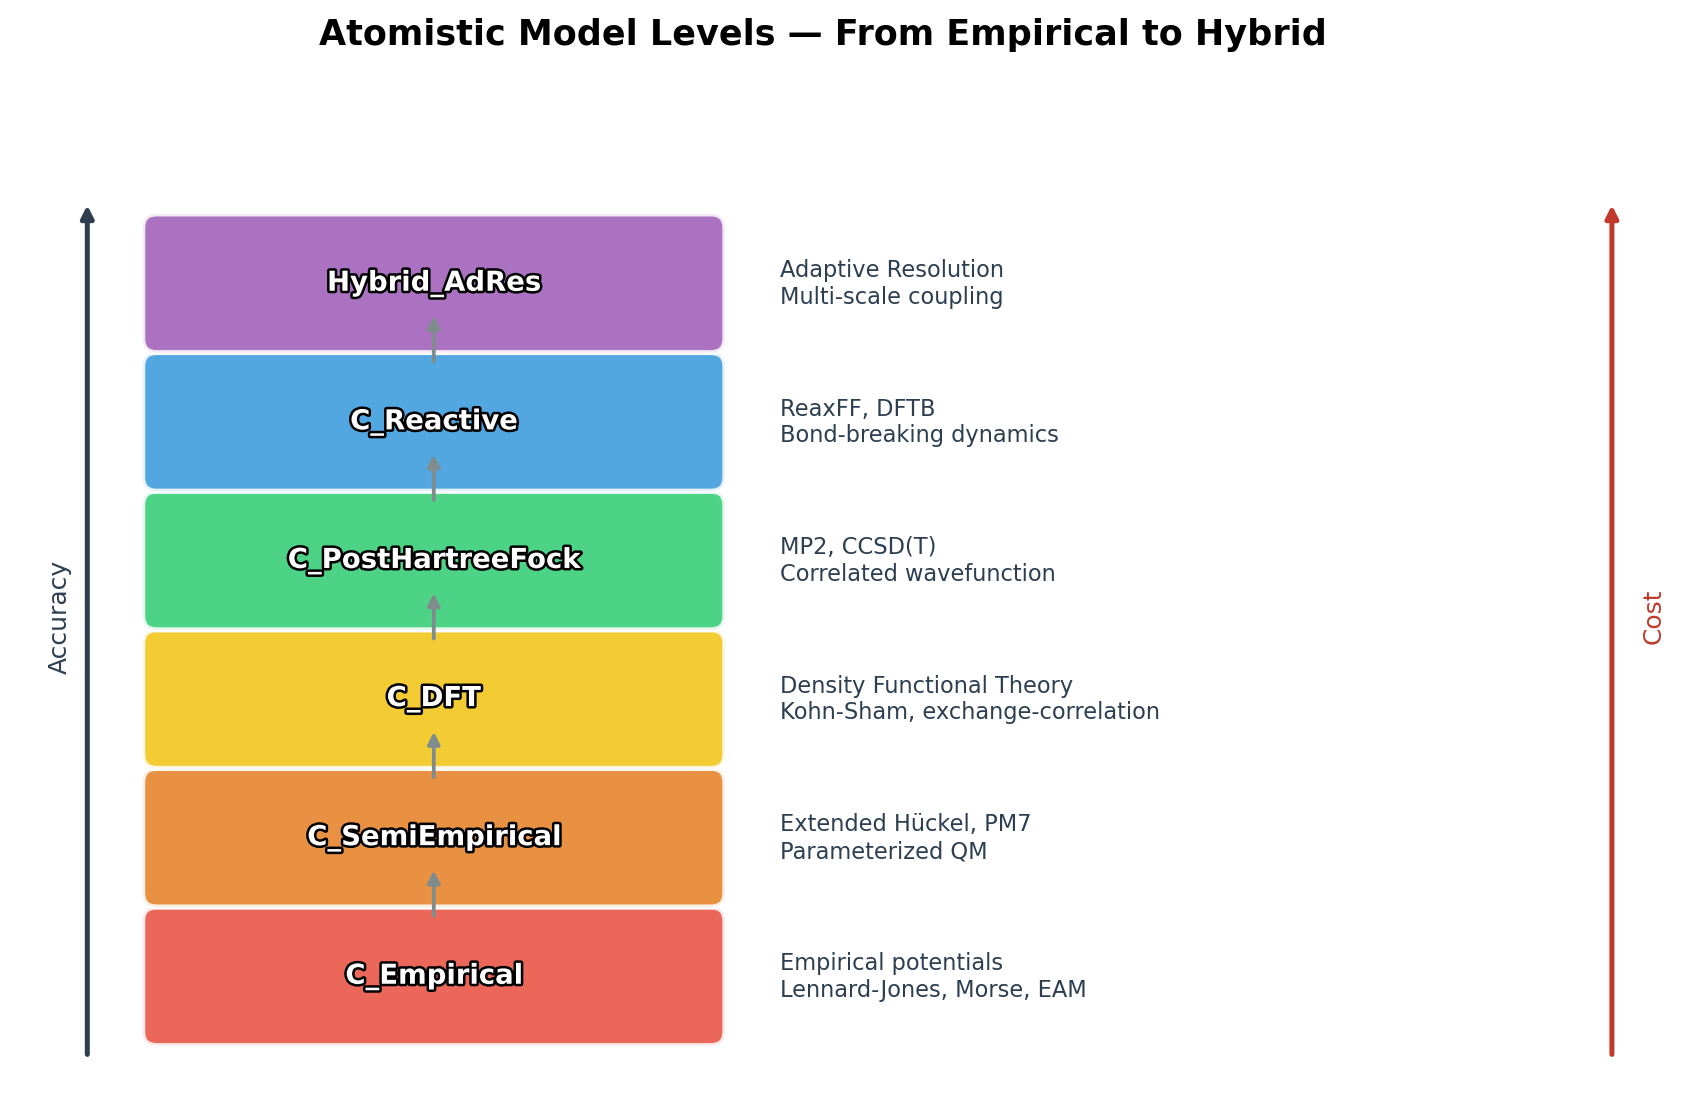
\includegraphics[width=0.85\textwidth]{overview_model_levels.png}
\caption{Model levels from empirical to hybrid adaptive resolution.}
\end{figure}

\subsection{Part III: Atomistic Engine and Datasets ($\sim$70 pages)}

\begin{center}
\renewcommand{\arraystretch}{1.2}
\begin{tabular}{lrl}
\toprule
\textbf{Document File} & \textbf{Pages} & \textbf{Key Topics} \\
\midrule
\texttt{section\_state\_c\_revised\_notation}         & 12 & $S_0 \to S_f$ transform, \texttt{evolve()} \\
\texttt{section\_emergence\_dataset\_1}               &  9 & Anisotropy, isomer falls \\
\texttt{deep\_research\_visual\_studies}               & 17 & 4-phase deep research engine \\
\texttt{section\_organometallic\_folding\_adsorption}  & 12 & Folding, surface adsorption \\
\texttt{section\_32bit\_hourglass\_lookglass}          &  9 & Precision analysis \\
\texttt{section\_petalized\_compute\_allocation}       &  7 & Resource scheduling \\
\texttt{section\_universal\_reaction\_engine}          &  4 & Generic reaction driver \\
\bottomrule
\end{tabular}
\end{center}

\begin{figure}[H]
\centering
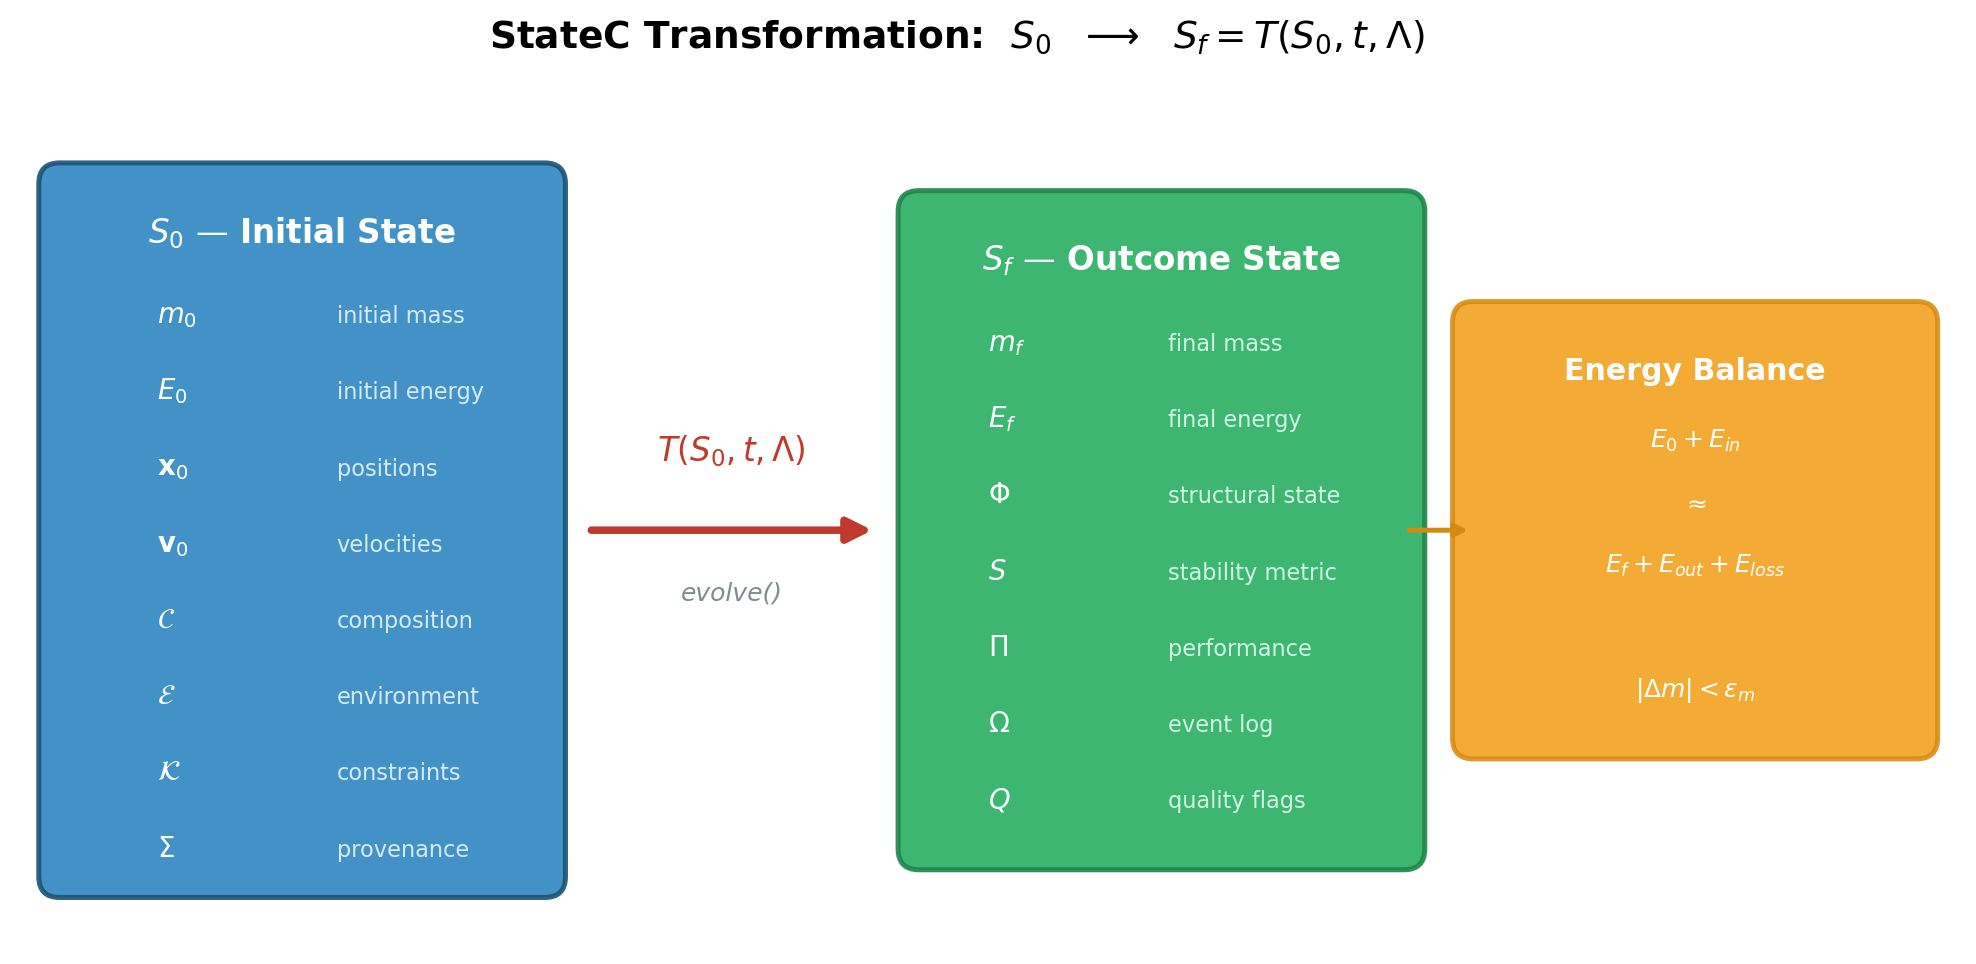
\includegraphics[width=0.92\textwidth]{overview_statec_flow.png}
\caption{StateC transformation: $S_0$ evolves to $S_f = T(S_0, t, \Lambda)$ with energy bookkeeping.}
\end{figure}

\begin{figure}[H]
\centering
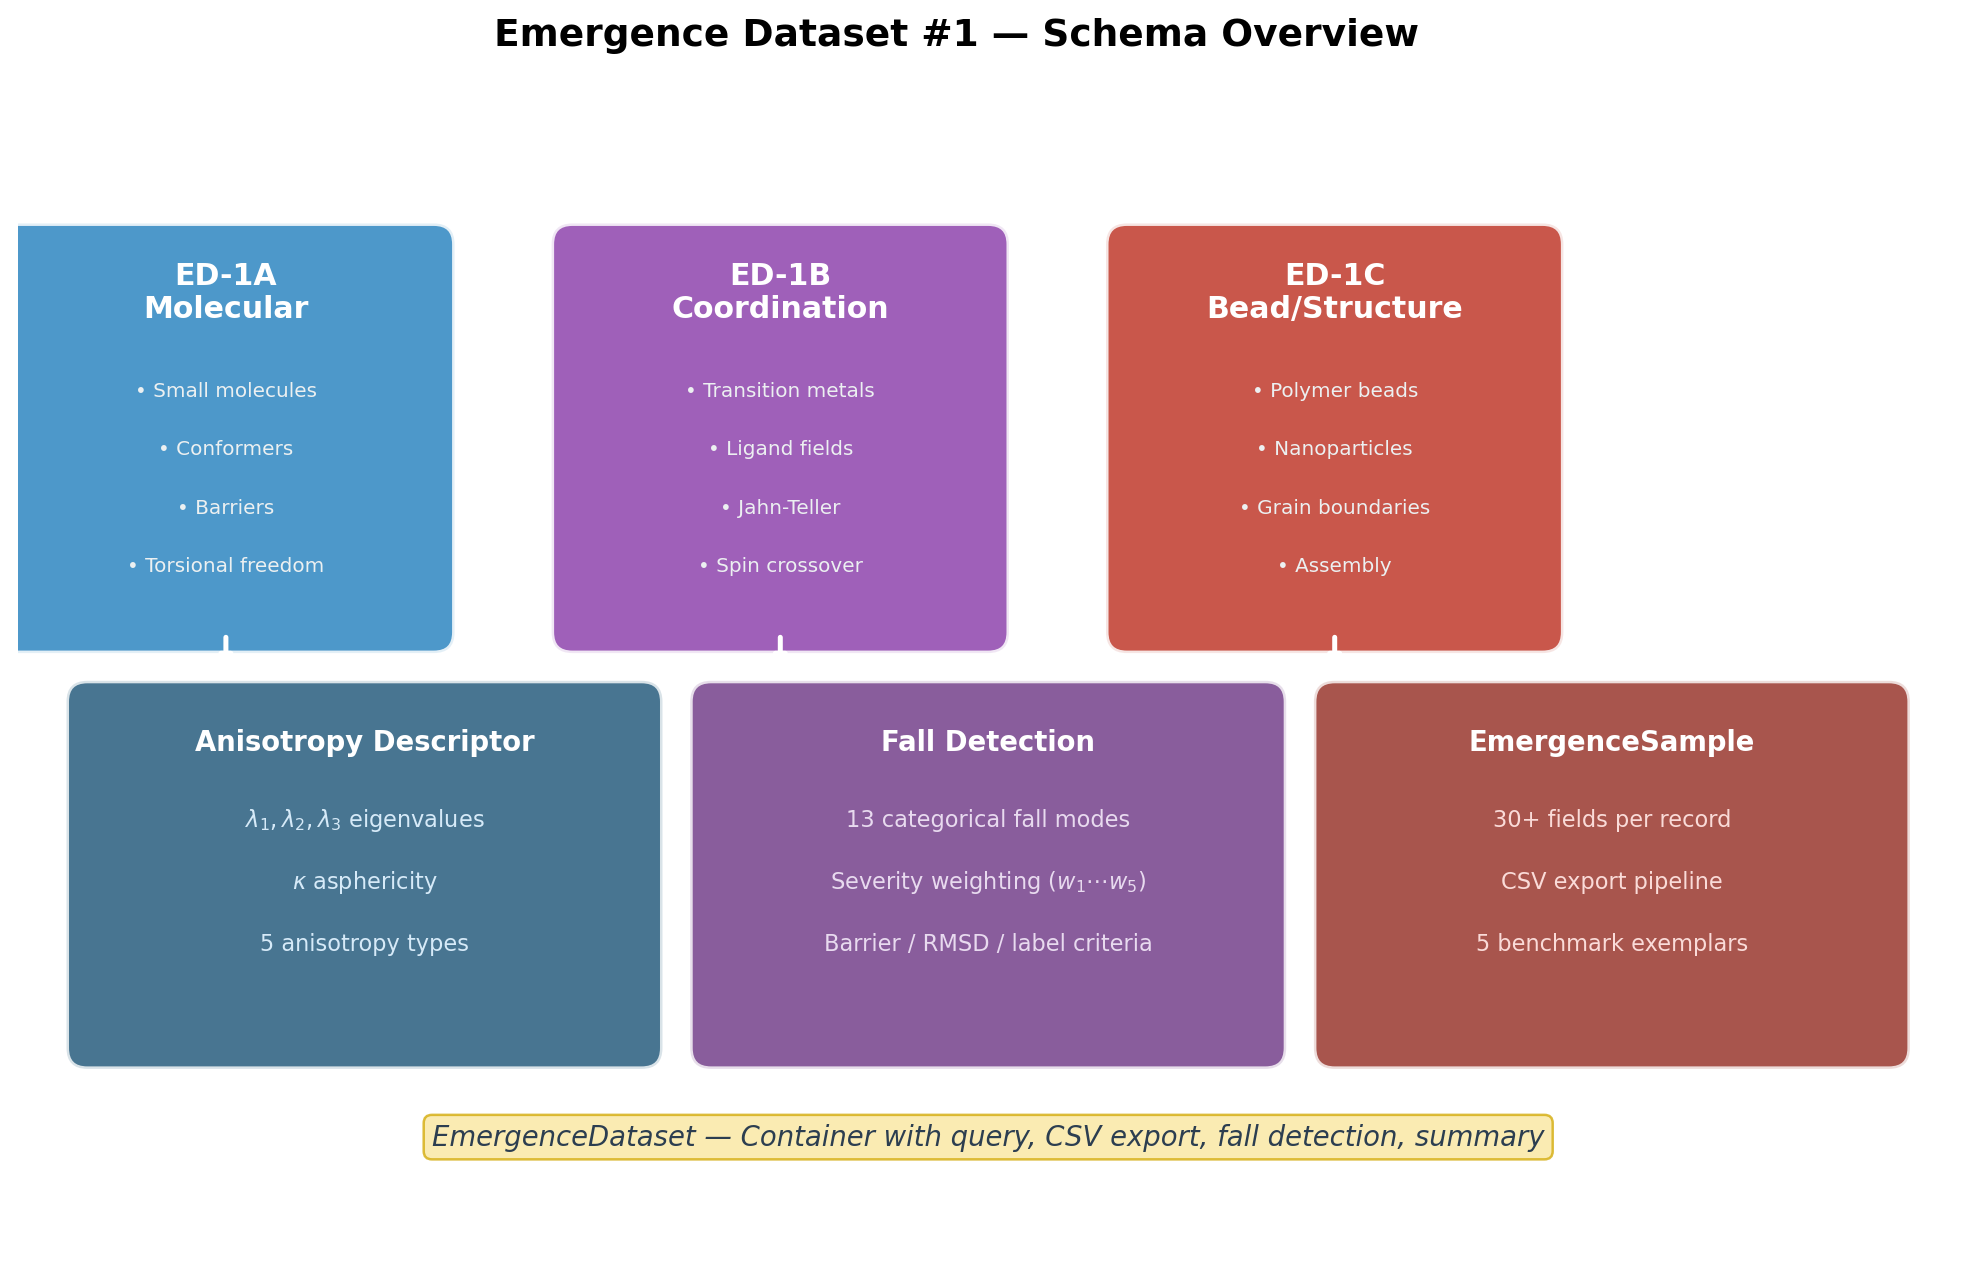
\includegraphics[width=0.92\textwidth]{overview_emergence_schema.png}
\caption{Emergence Dataset \#1 schema: three families, anisotropy detection, fall severity.}
\end{figure}

\begin{figure}[H]
\centering
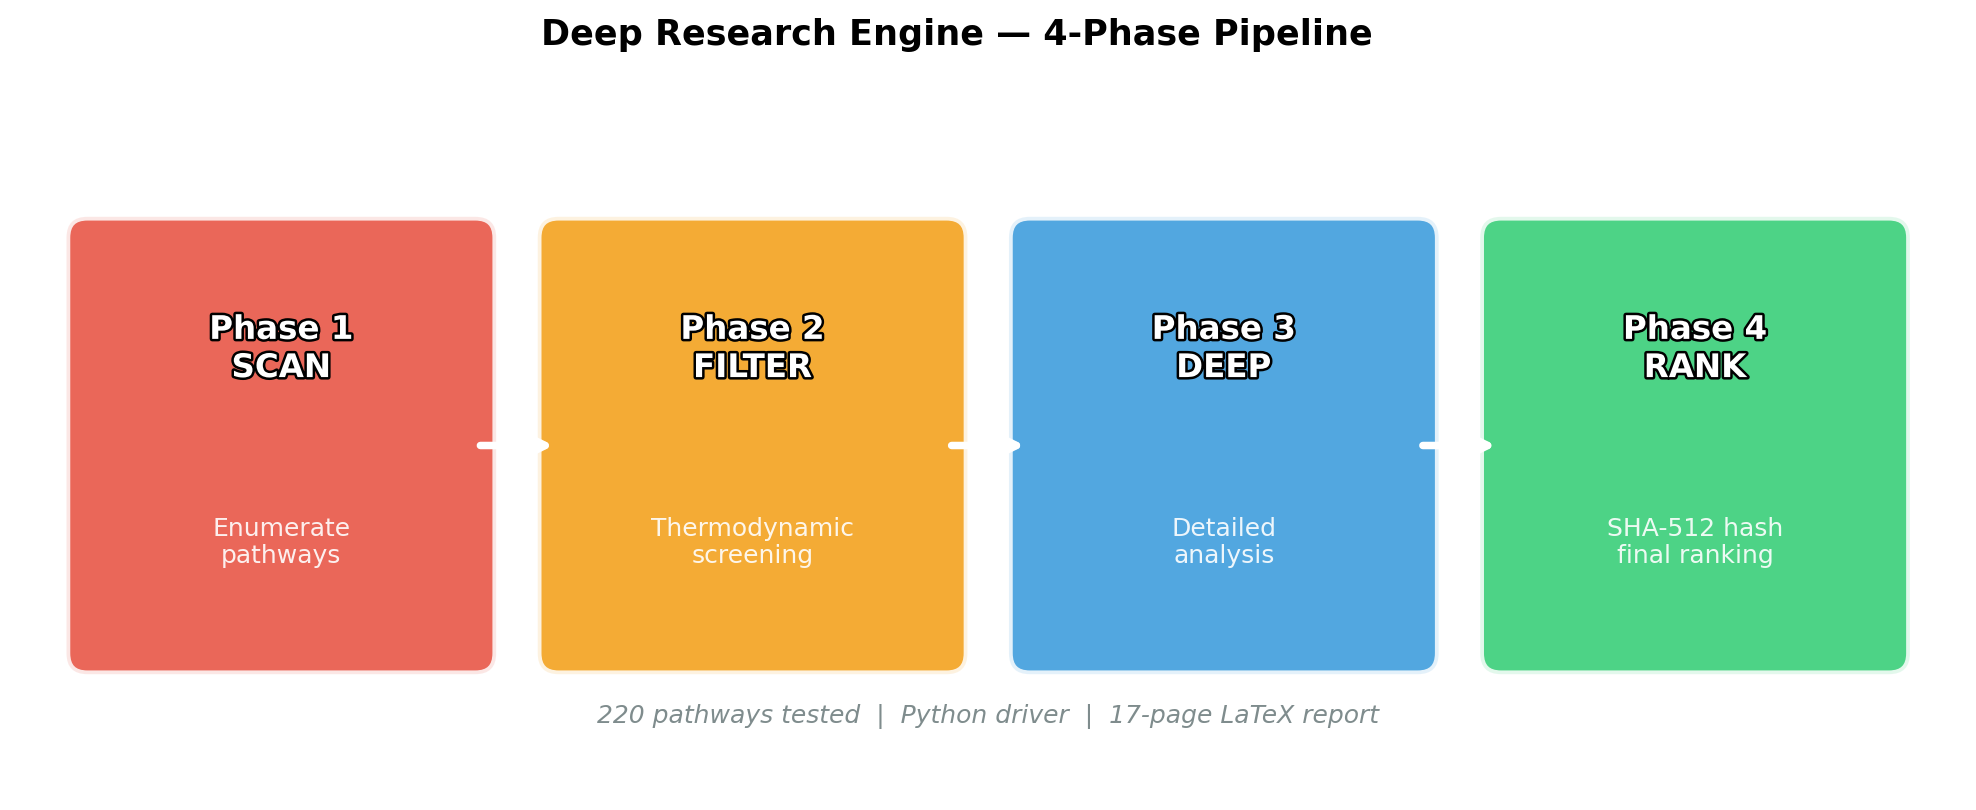
\includegraphics[width=0.92\textwidth]{overview_deep_research_phases.png}
\caption{4-phase deep research pipeline: Scan $\to$ Filter $\to$ Deep $\to$ Rank.}
\end{figure}

\subsection{Part IV: Electrohydrodynamics (18 pages)}

\begin{center}
\renewcommand{\arraystretch}{1.2}
\begin{tabular}{lrl}
\toprule
\textbf{Document File} & \textbf{Pages} & \textbf{Key Topics} \\
\midrule
\texttt{ehd\_theory} & 18 & EHD coupling, 26 headers, 36 tests \\
\bottomrule
\end{tabular}
\end{center}

\begin{figure}[H]
\centering
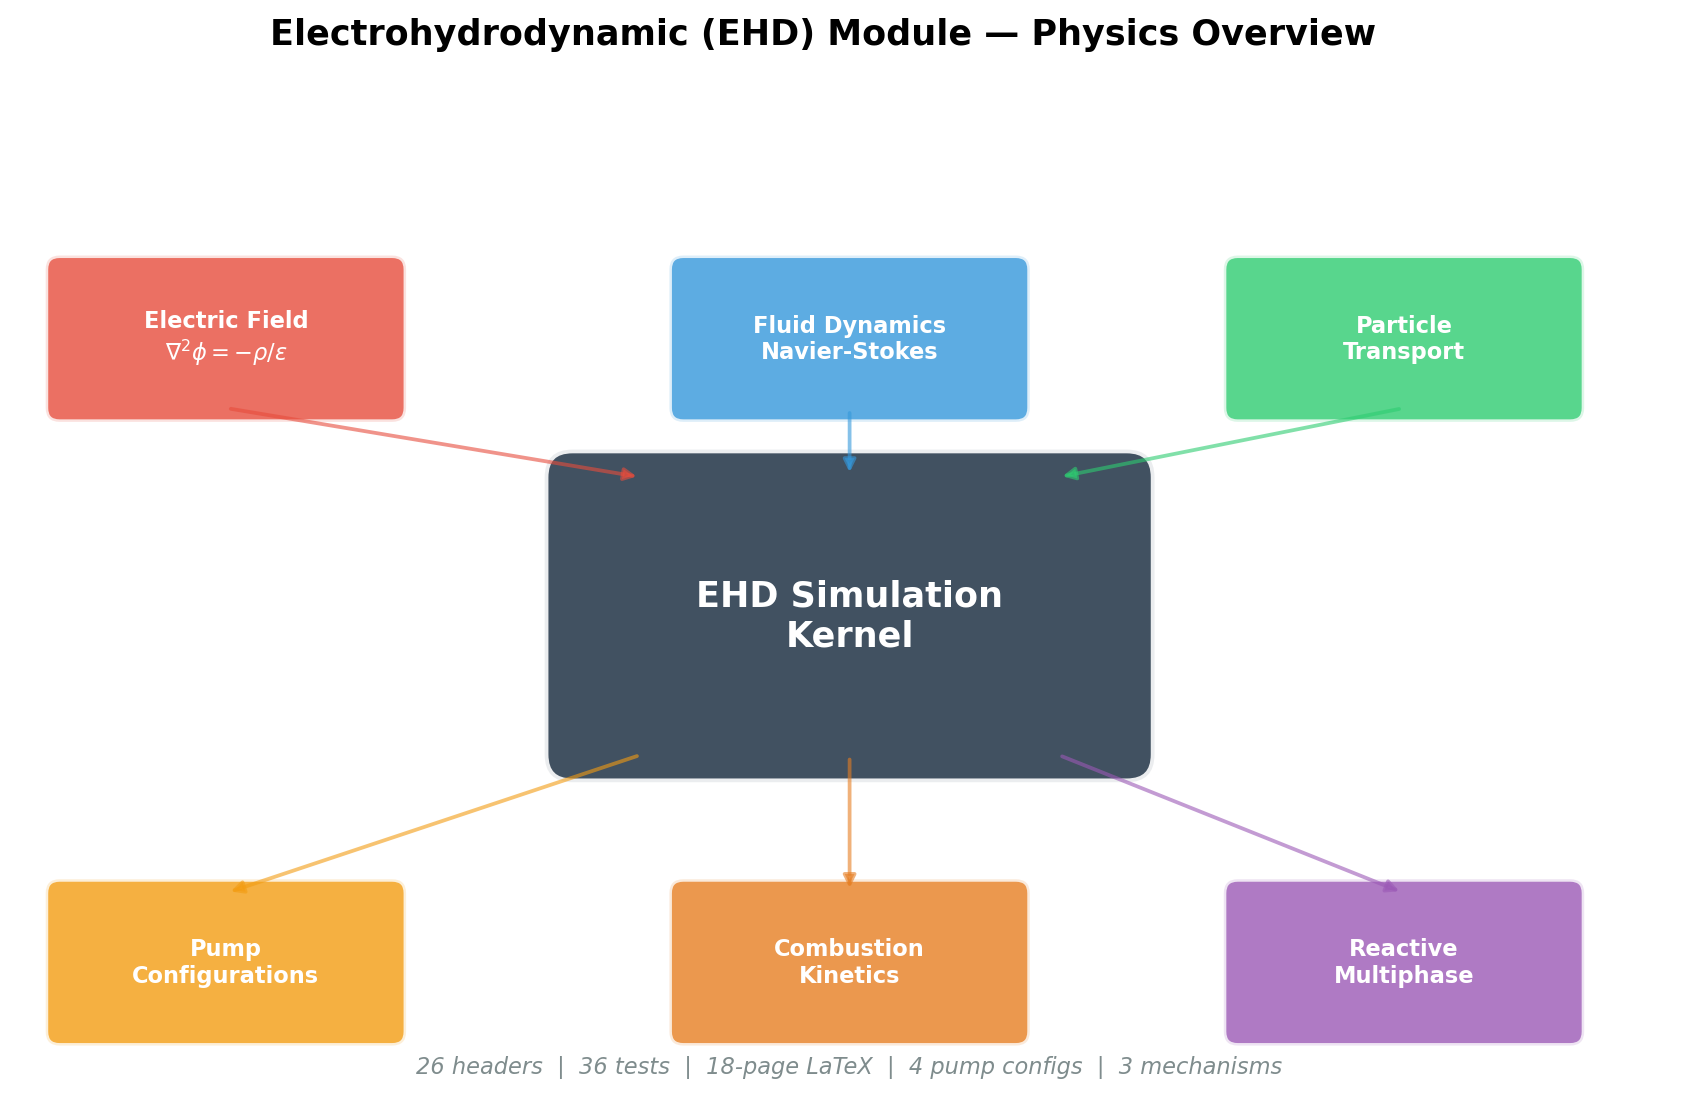
\includegraphics[width=0.85\textwidth]{overview_ehd_summary.png}
\caption{EHD module: six coupled physics sub-modules.}
\end{figure}

\subsection{Part V: Visualization and Inspection (115 pages)}

\begin{center}
\renewcommand{\arraystretch}{1.2}
\begin{tabular}{lrl}
\toprule
\textbf{Document File} & \textbf{Pages} & \textbf{Key Topics} \\
\midrule
\texttt{section\_visualization\_inspection} & 115 & 84 figures, 15 inspection points \\
\addlinespace
\texttt{section\_viz\_dualport} & 15 & Phase 16: dual-port 3D live rendering,
                                       atom record $\mathcal{A}_i(t)$, port 9999
                                       atomic view, port 10001 analysis view,
                                       MB speed distribution, candidate panel,
                                       wire protocol, continuous sim launcher \\
\bottomrule
\end{tabular}
\end{center}

This is the largest single document, containing rendered 2D/3D molecular views,
bond topology diagrams, XRD patterns, flame dashboards, RDF curves, stress--strain
analysis, and more.

\texttt{section\_viz\_dualport} documents the Phase~16 dual-port live rendering
architecture: a fast tactical viewer (port 9999) for the live atomistic state and
a heavy analysis viewer (port 10001) for historical metrics, property panels,
candidate comparison, and 3D crystal scenes.

\subsection{Part VI: Methodology and Reports ($\sim$40 pages)}

\begin{center}
\renewcommand{\arraystretch}{1.2}
\begin{tabular}{lrl}
\toprule
\textbf{Document File} & \textbf{Pages} & \textbf{Key Topics} \\
\midrule
\texttt{ALPHA\_MODEL\_BOOKLET}   &  8 & Alpha polarizability model \\
\texttt{METHODOLOGY\_12PAGE}     &  7 & Condensed methodology \\
\texttt{METHODOLOGY\_2PAGE}      &  2 & Executive summary \\
\texttt{xyz\_file\_formats}      & 11 & XYZ/extended format spec \\
\texttt{section\_final\_statement} & 12 & Thesis conclusion \\
\bottomrule
\end{tabular}
\end{center}

\subsection{Part VII: Infrastructure ($\sim$9 pages)}

\begin{center}
\renewcommand{\arraystretch}{1.2}
\begin{tabular}{lrl}
\toprule
\textbf{Document File} & \textbf{Pages} & \textbf{Key Topics} \\
\midrule
\texttt{section\_testing\_infrastructure} &  5 & CMake test groups 1--14 \\
\texttt{section\_phase\_reports}          &  4 & Development phase tracking \\
\bottomrule
\end{tabular}
\end{center}

\begin{figure}[H]
\centering
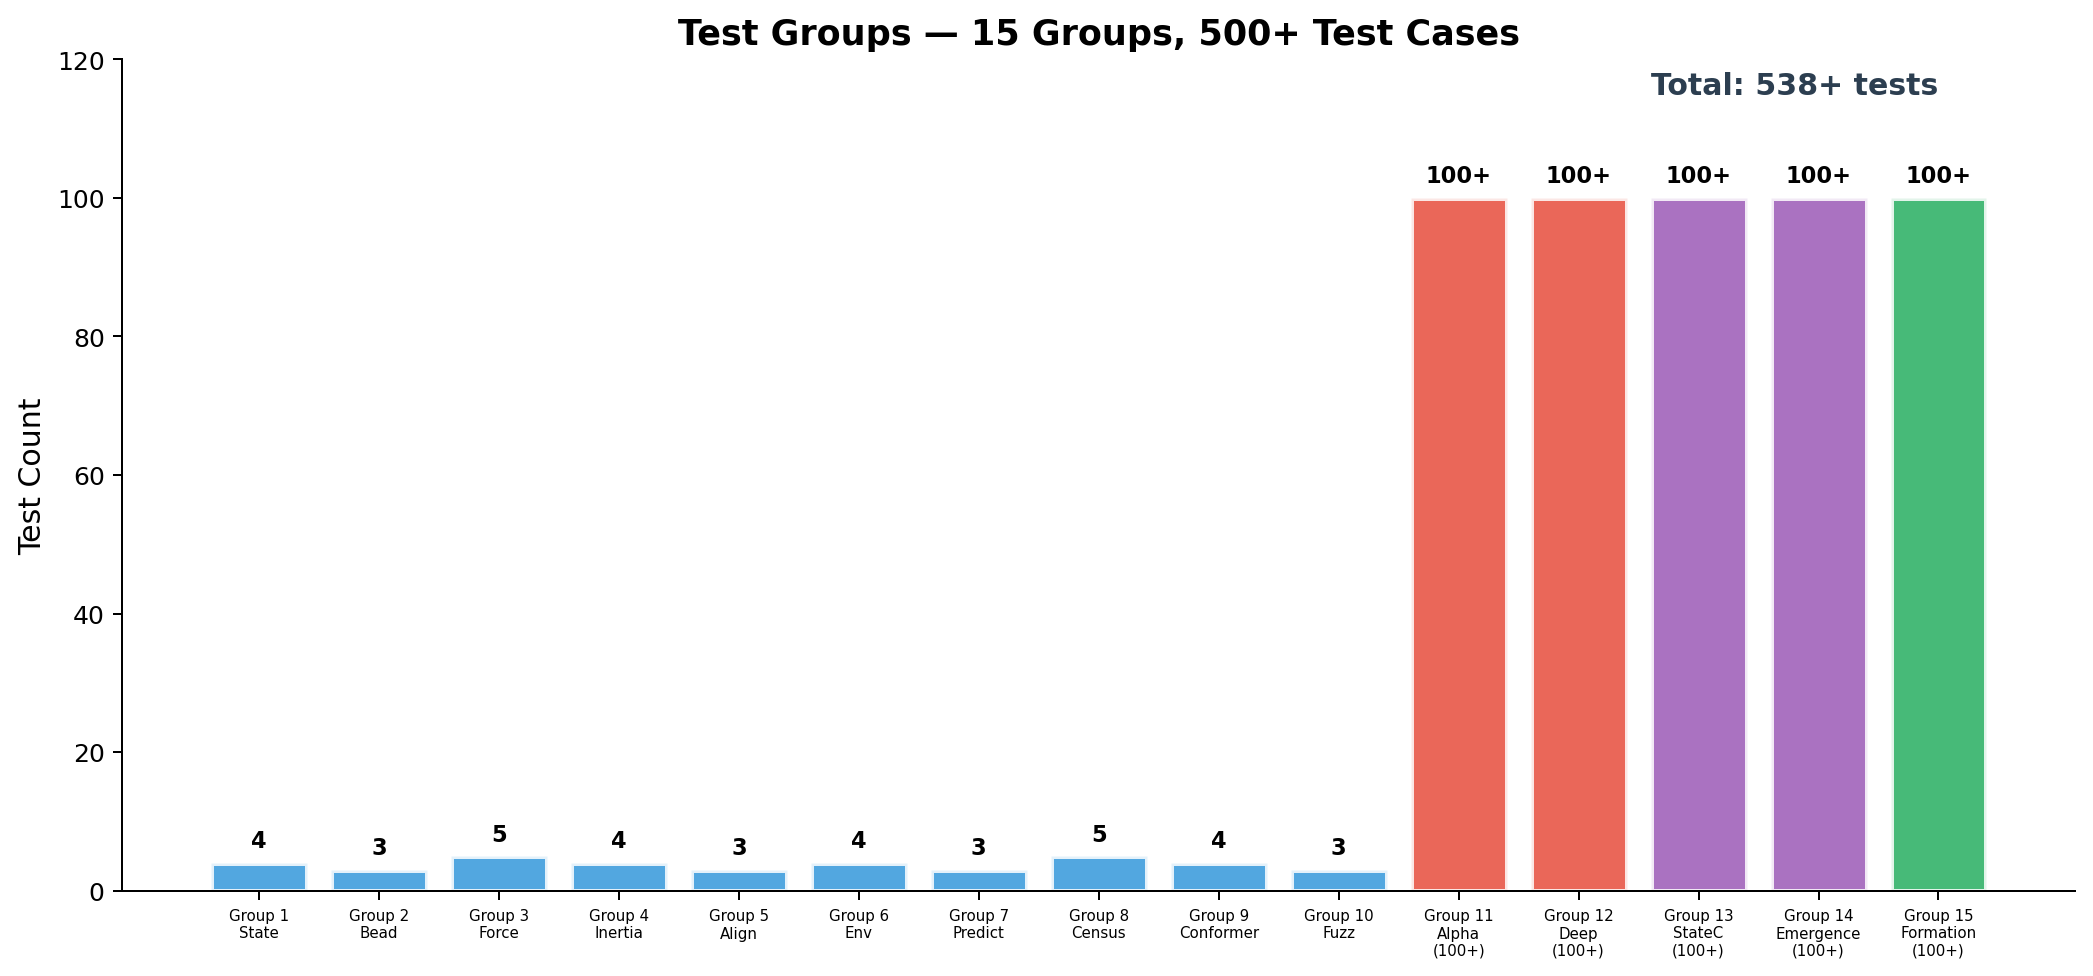
\includegraphics[width=0.85\textwidth]{overview_test_coverage.png}
\caption{Test coverage across 15 groups. Groups 11--15 each target 100+ tests (self-audit, validation, atomistic, emergence, formation/chemical/pipes).}
\end{figure}


% ════════════════════════════════════════════════════════════════════════════
\section{Figure Gallery Highlights}
% ════════════════════════════════════════════════════════════════════════════

The project contains \textbf{96 rendered PNG figures}: 84 molecular/analysis
figures generated by \texttt{render\_document\_figures.py} and 12 overview
diagrams generated by \texttt{render\_overview\_figures.py}.

\begin{figure}[H]
\centering
\begin{subfigure}[b]{0.30\textwidth}
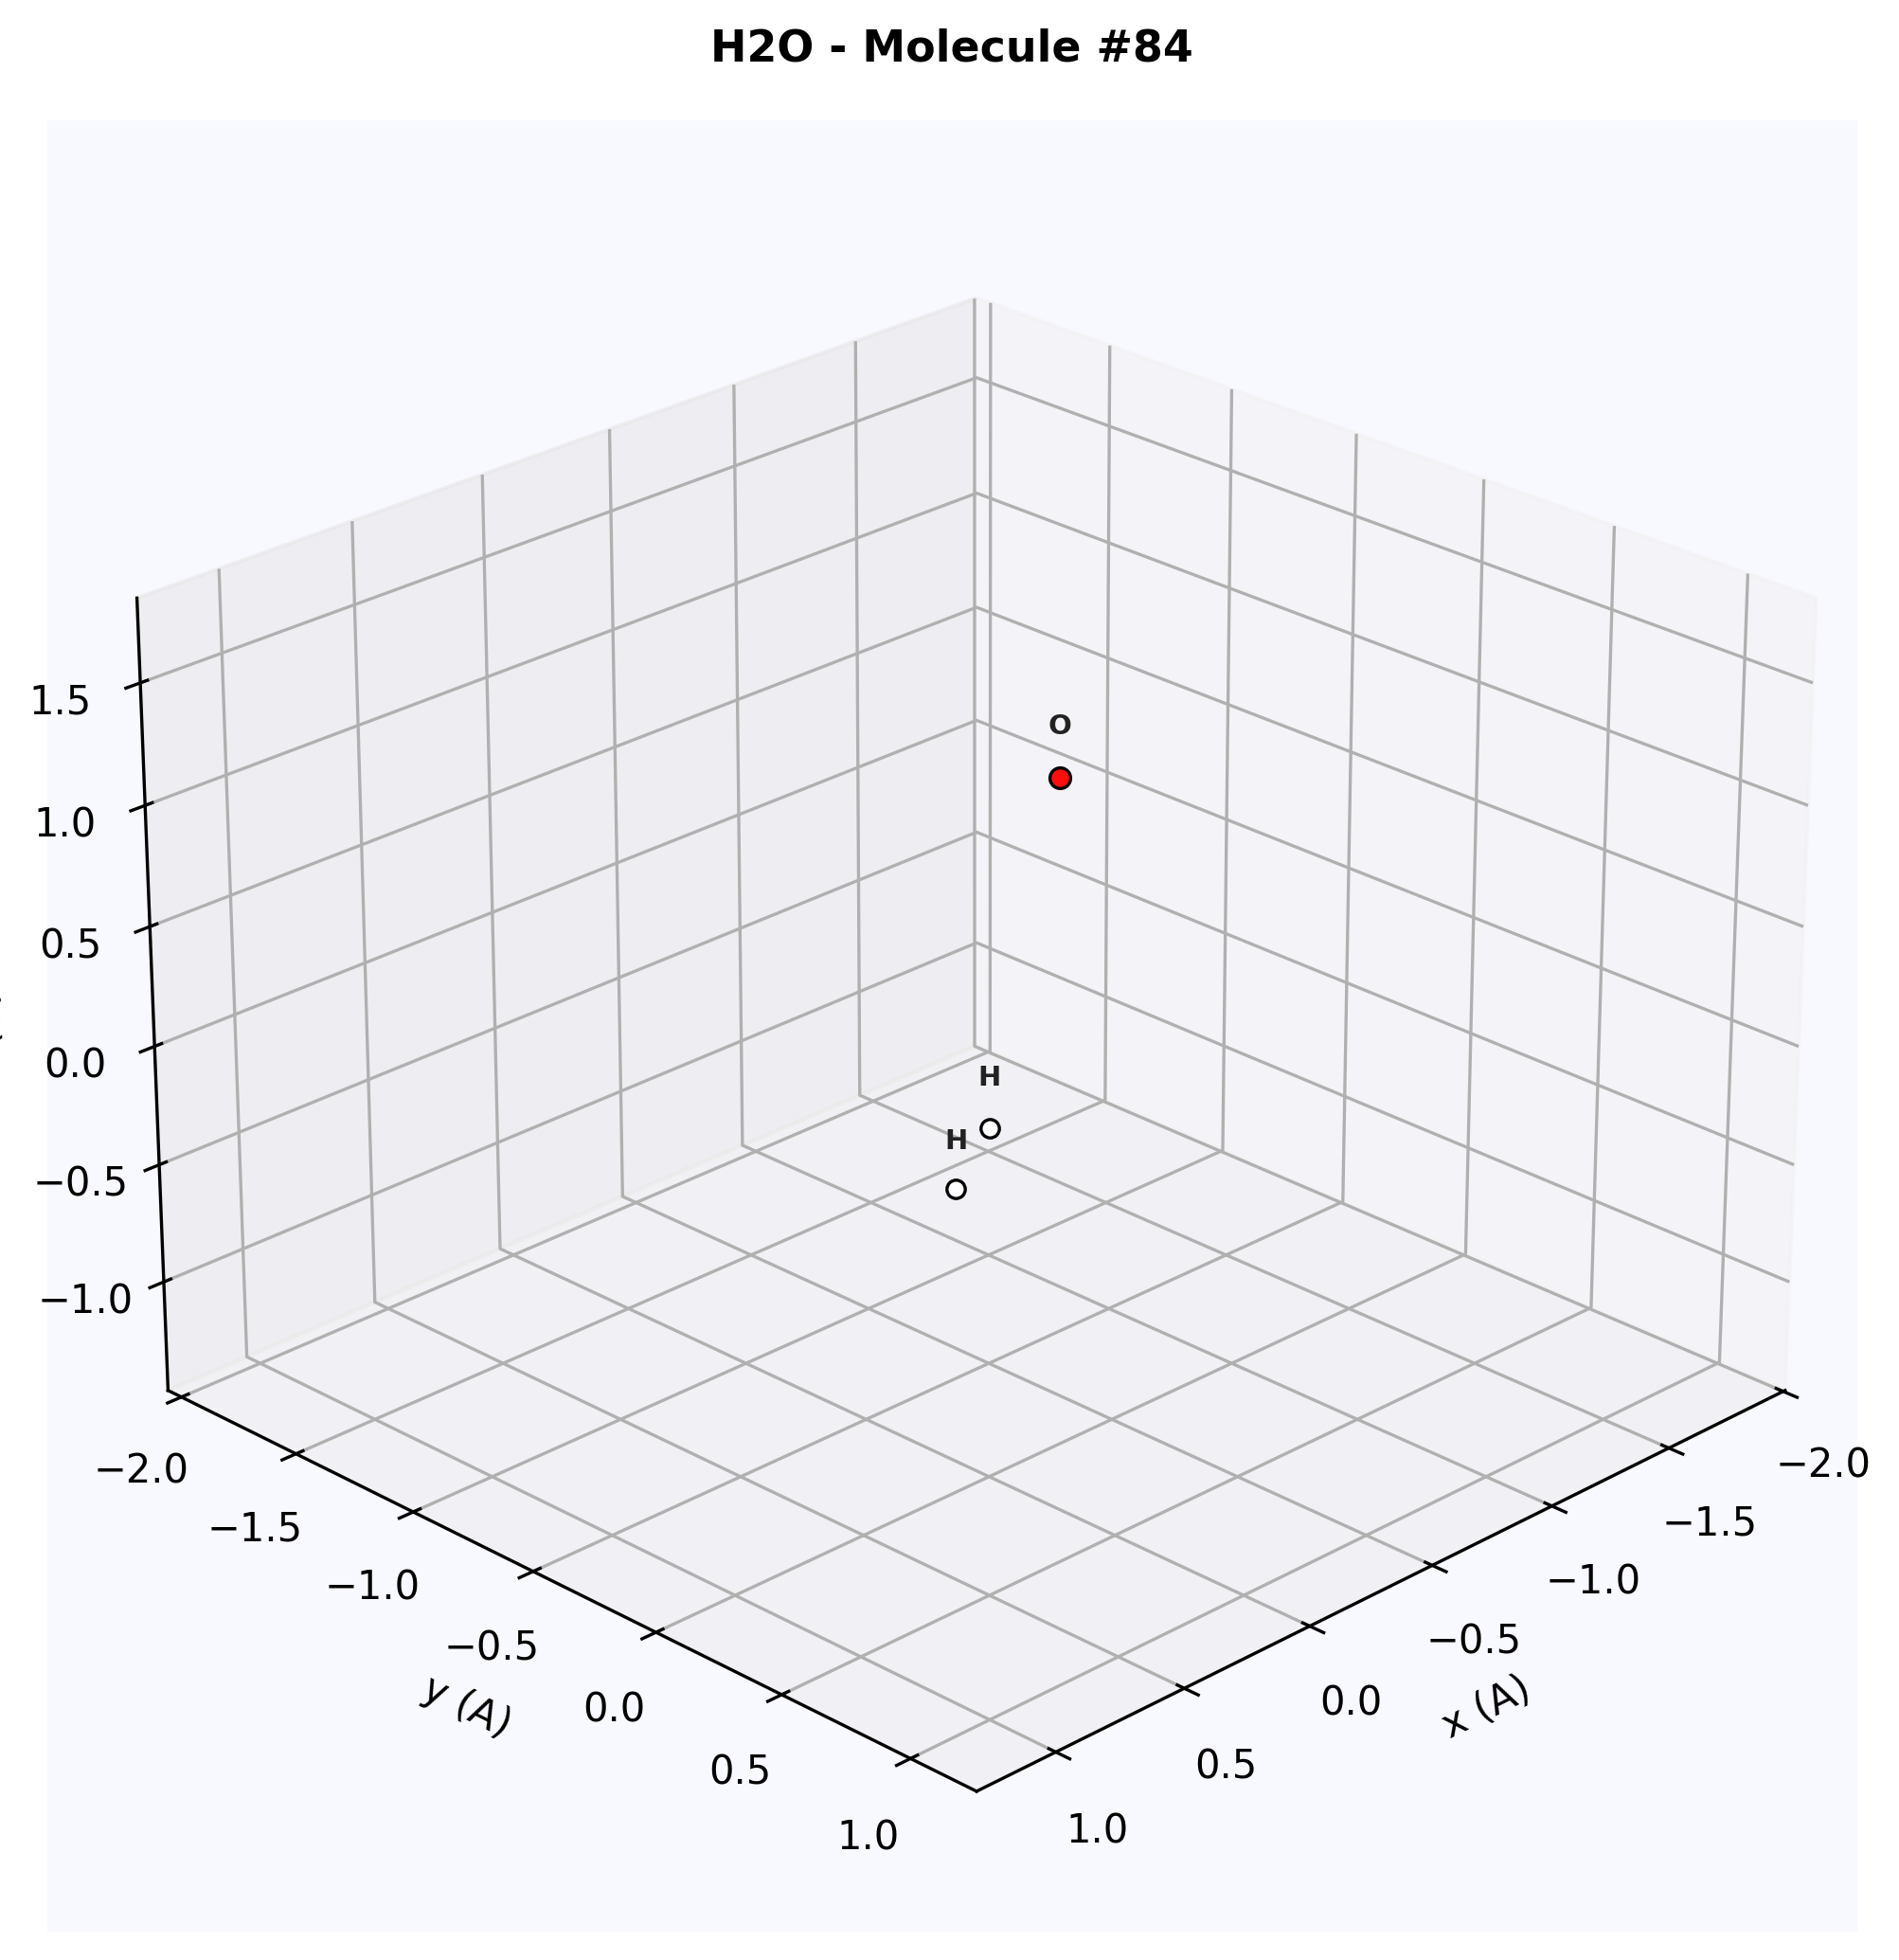
\includegraphics[width=\textwidth]{mol3d_H2O_84.png}
\caption{H$_2$O (3D)}
\end{subfigure}
\hfill
\begin{subfigure}[b]{0.30\textwidth}
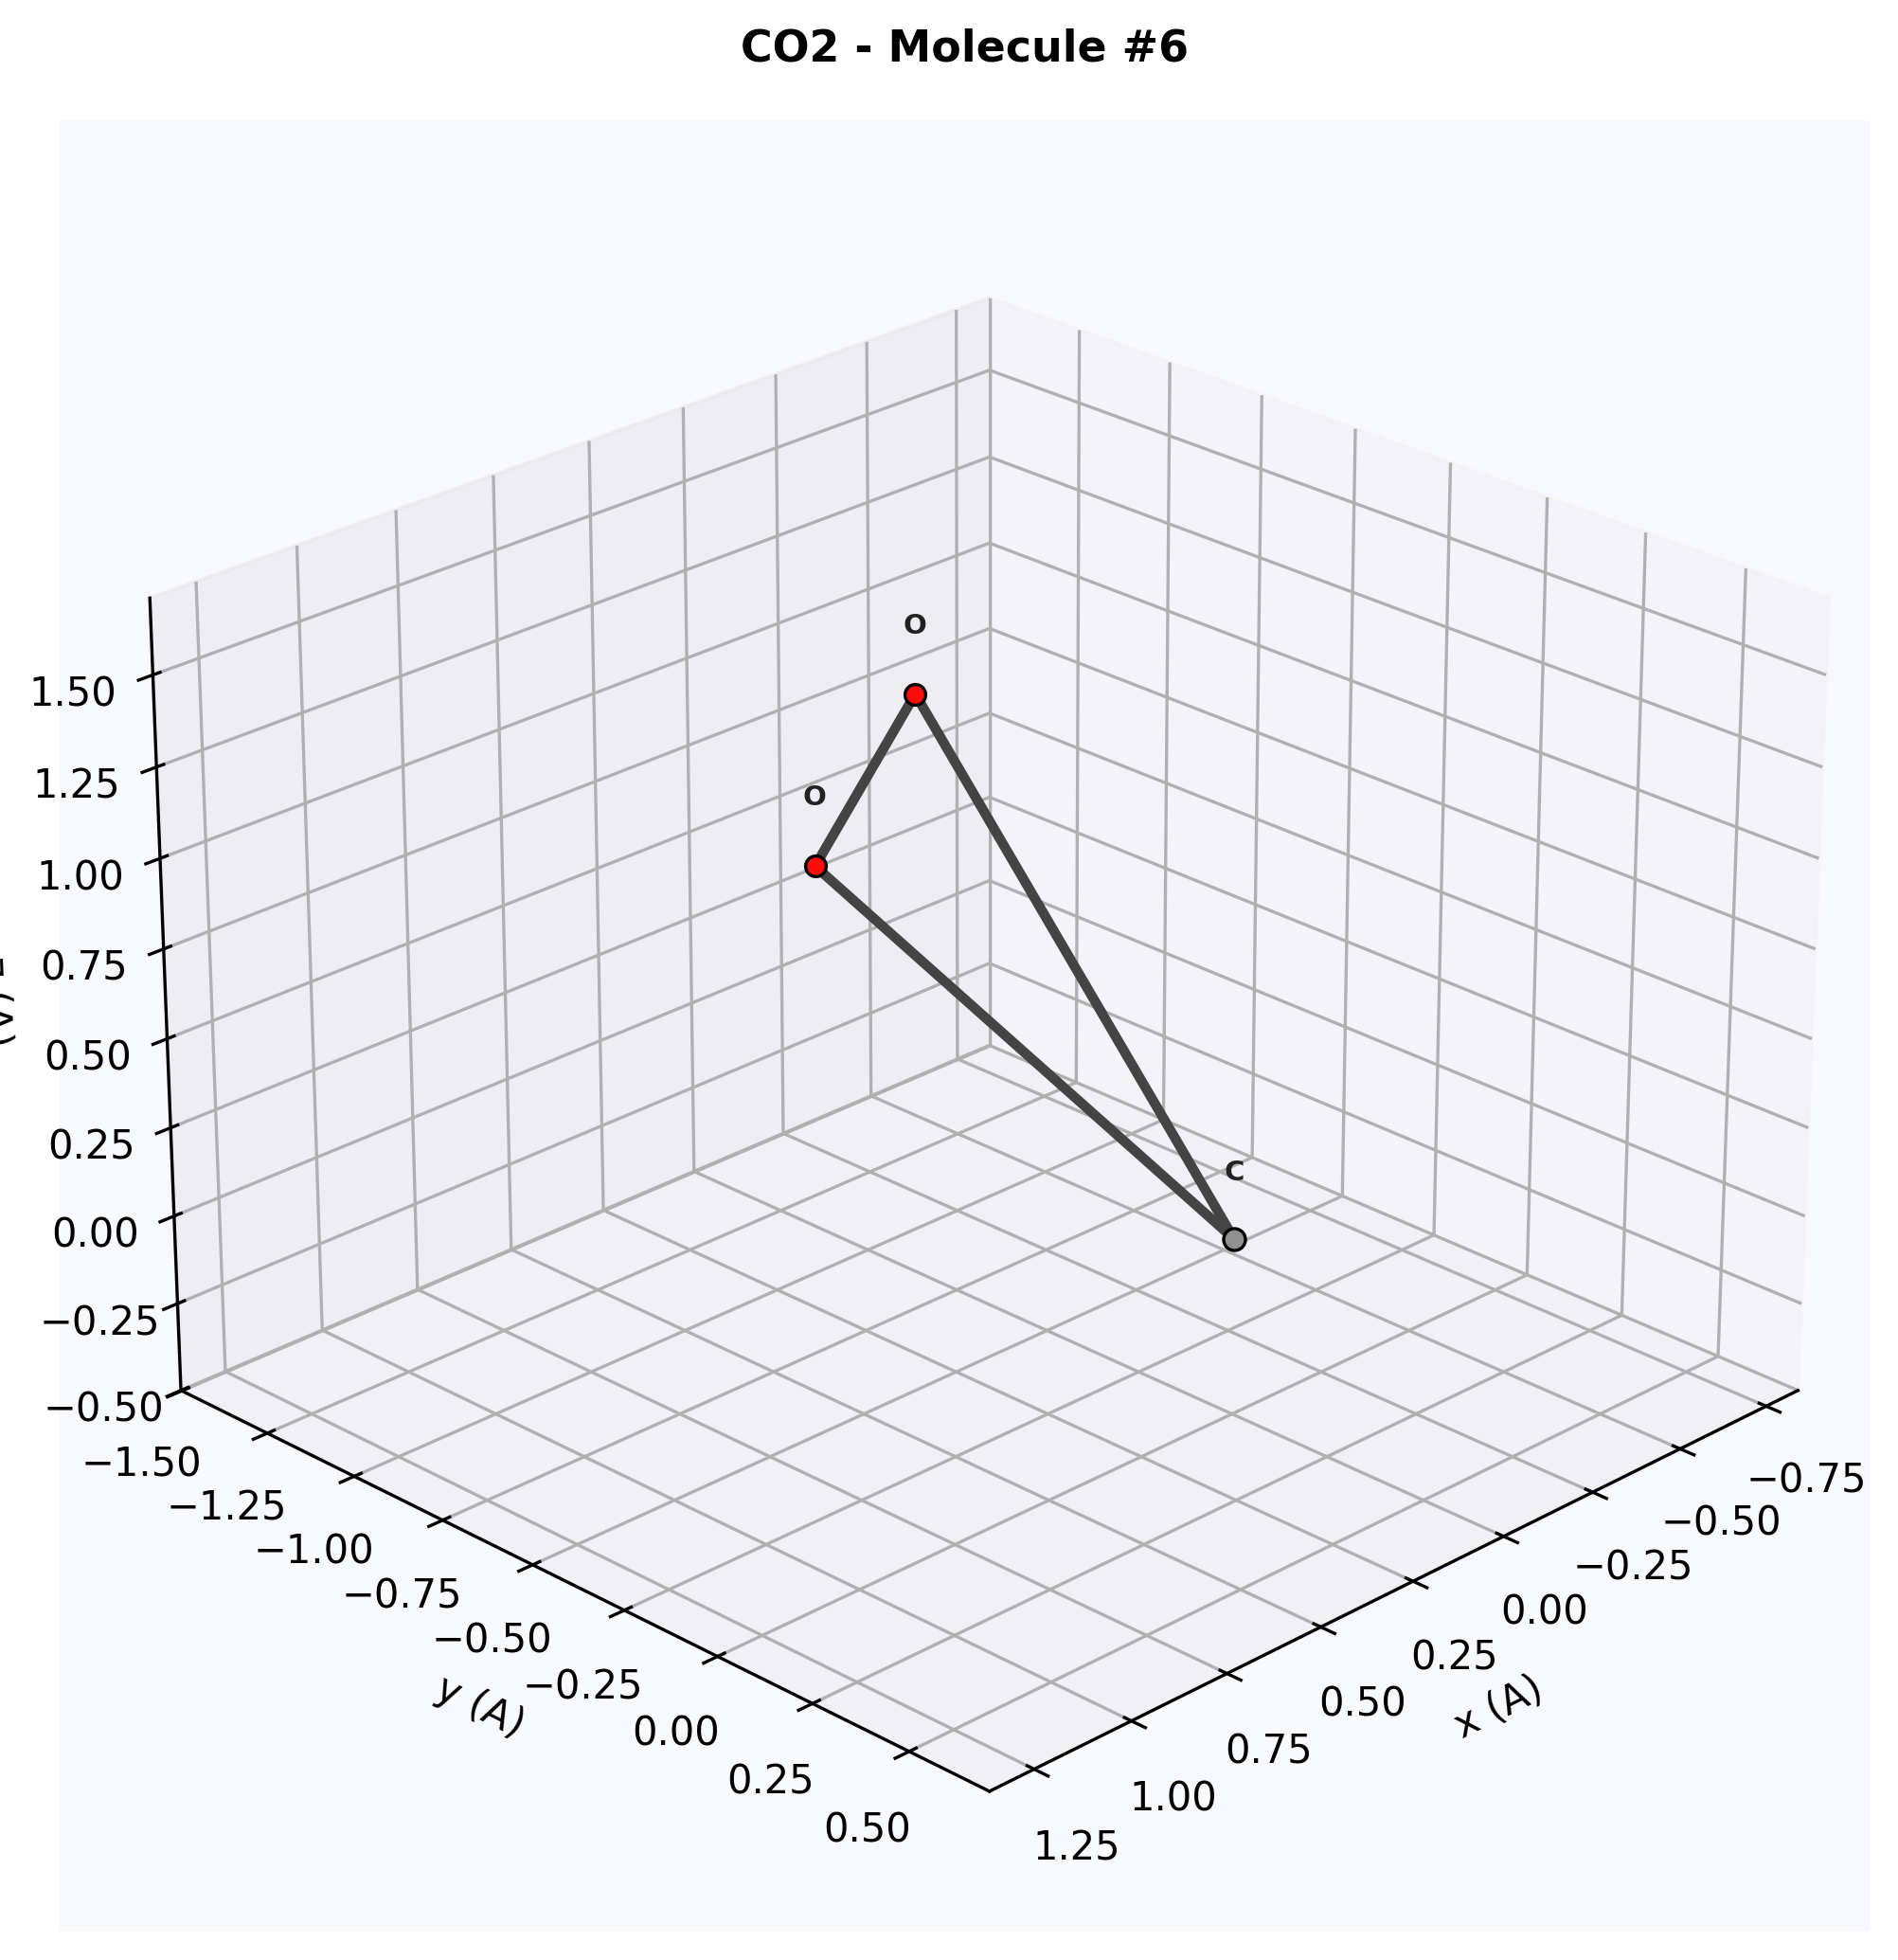
\includegraphics[width=\textwidth]{mol3d_CO2_6.png}
\caption{CO$_2$ (3D)}
\end{subfigure}
\hfill
\begin{subfigure}[b]{0.30\textwidth}
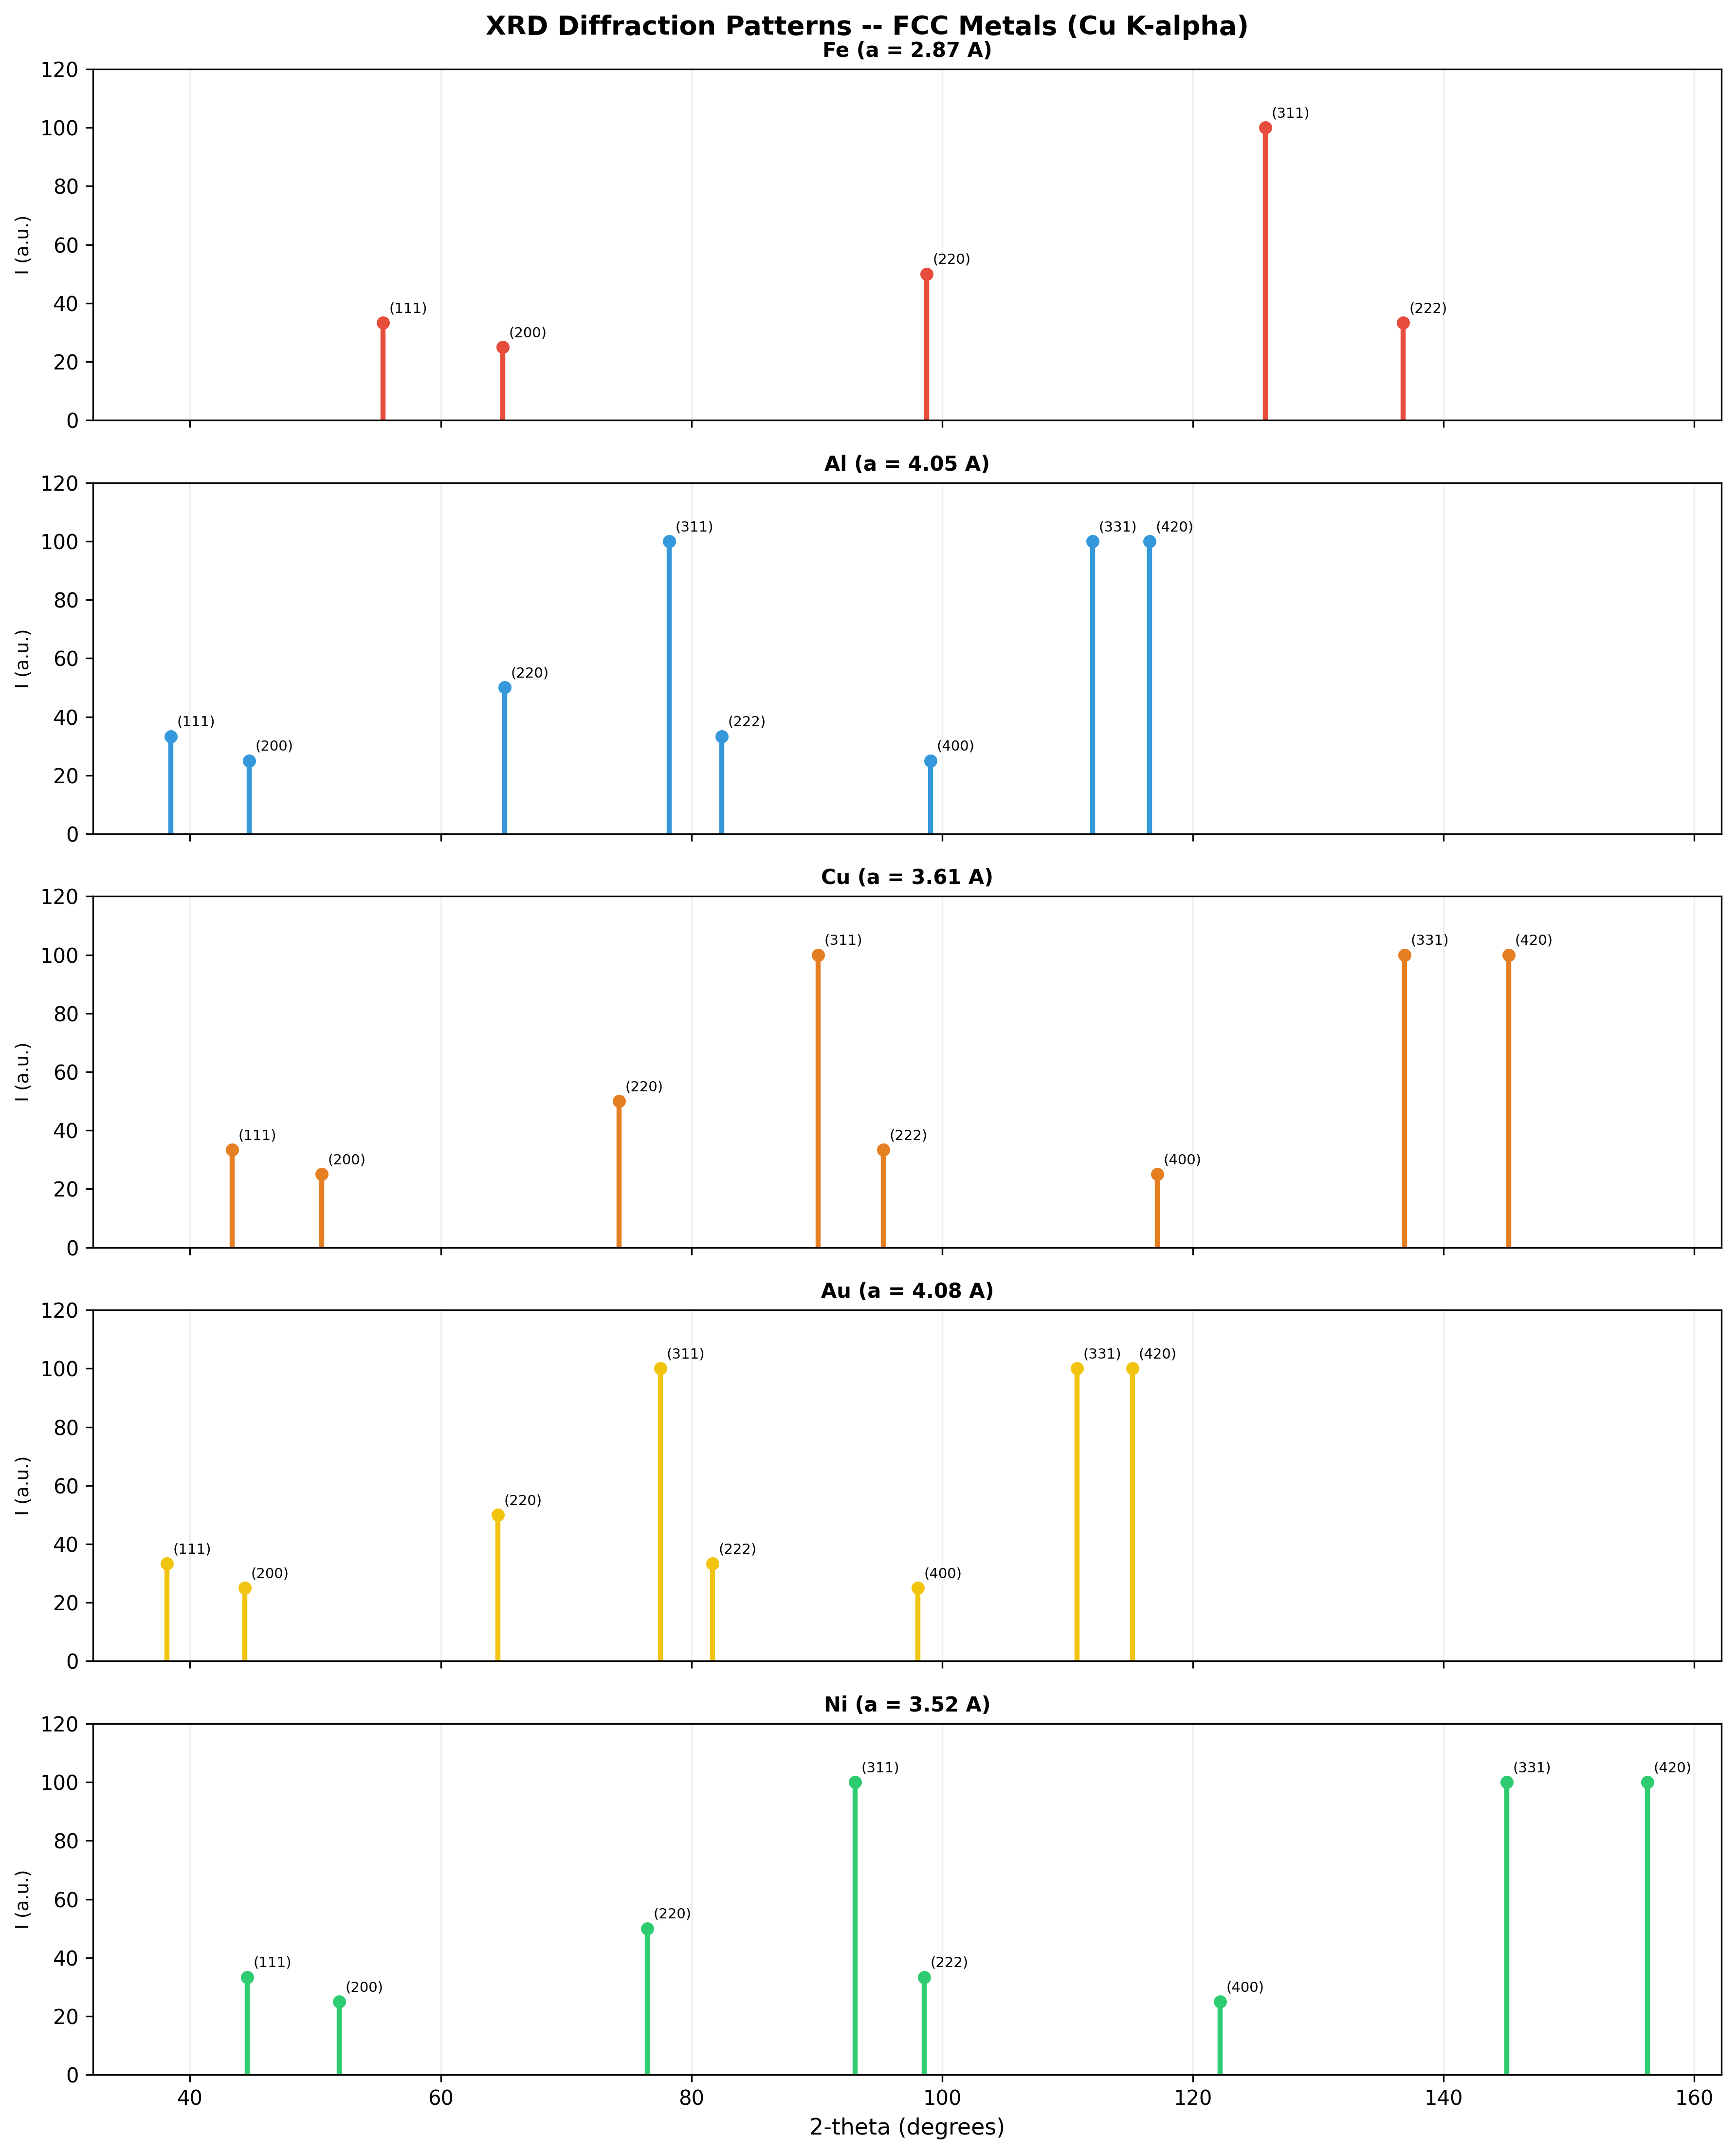
\includegraphics[width=\textwidth]{xrd_patterns.png}
\caption{XRD patterns}
\end{subfigure}
\end{figure}

\begin{figure}[H]
\centering
\begin{subfigure}[b]{0.30\textwidth}
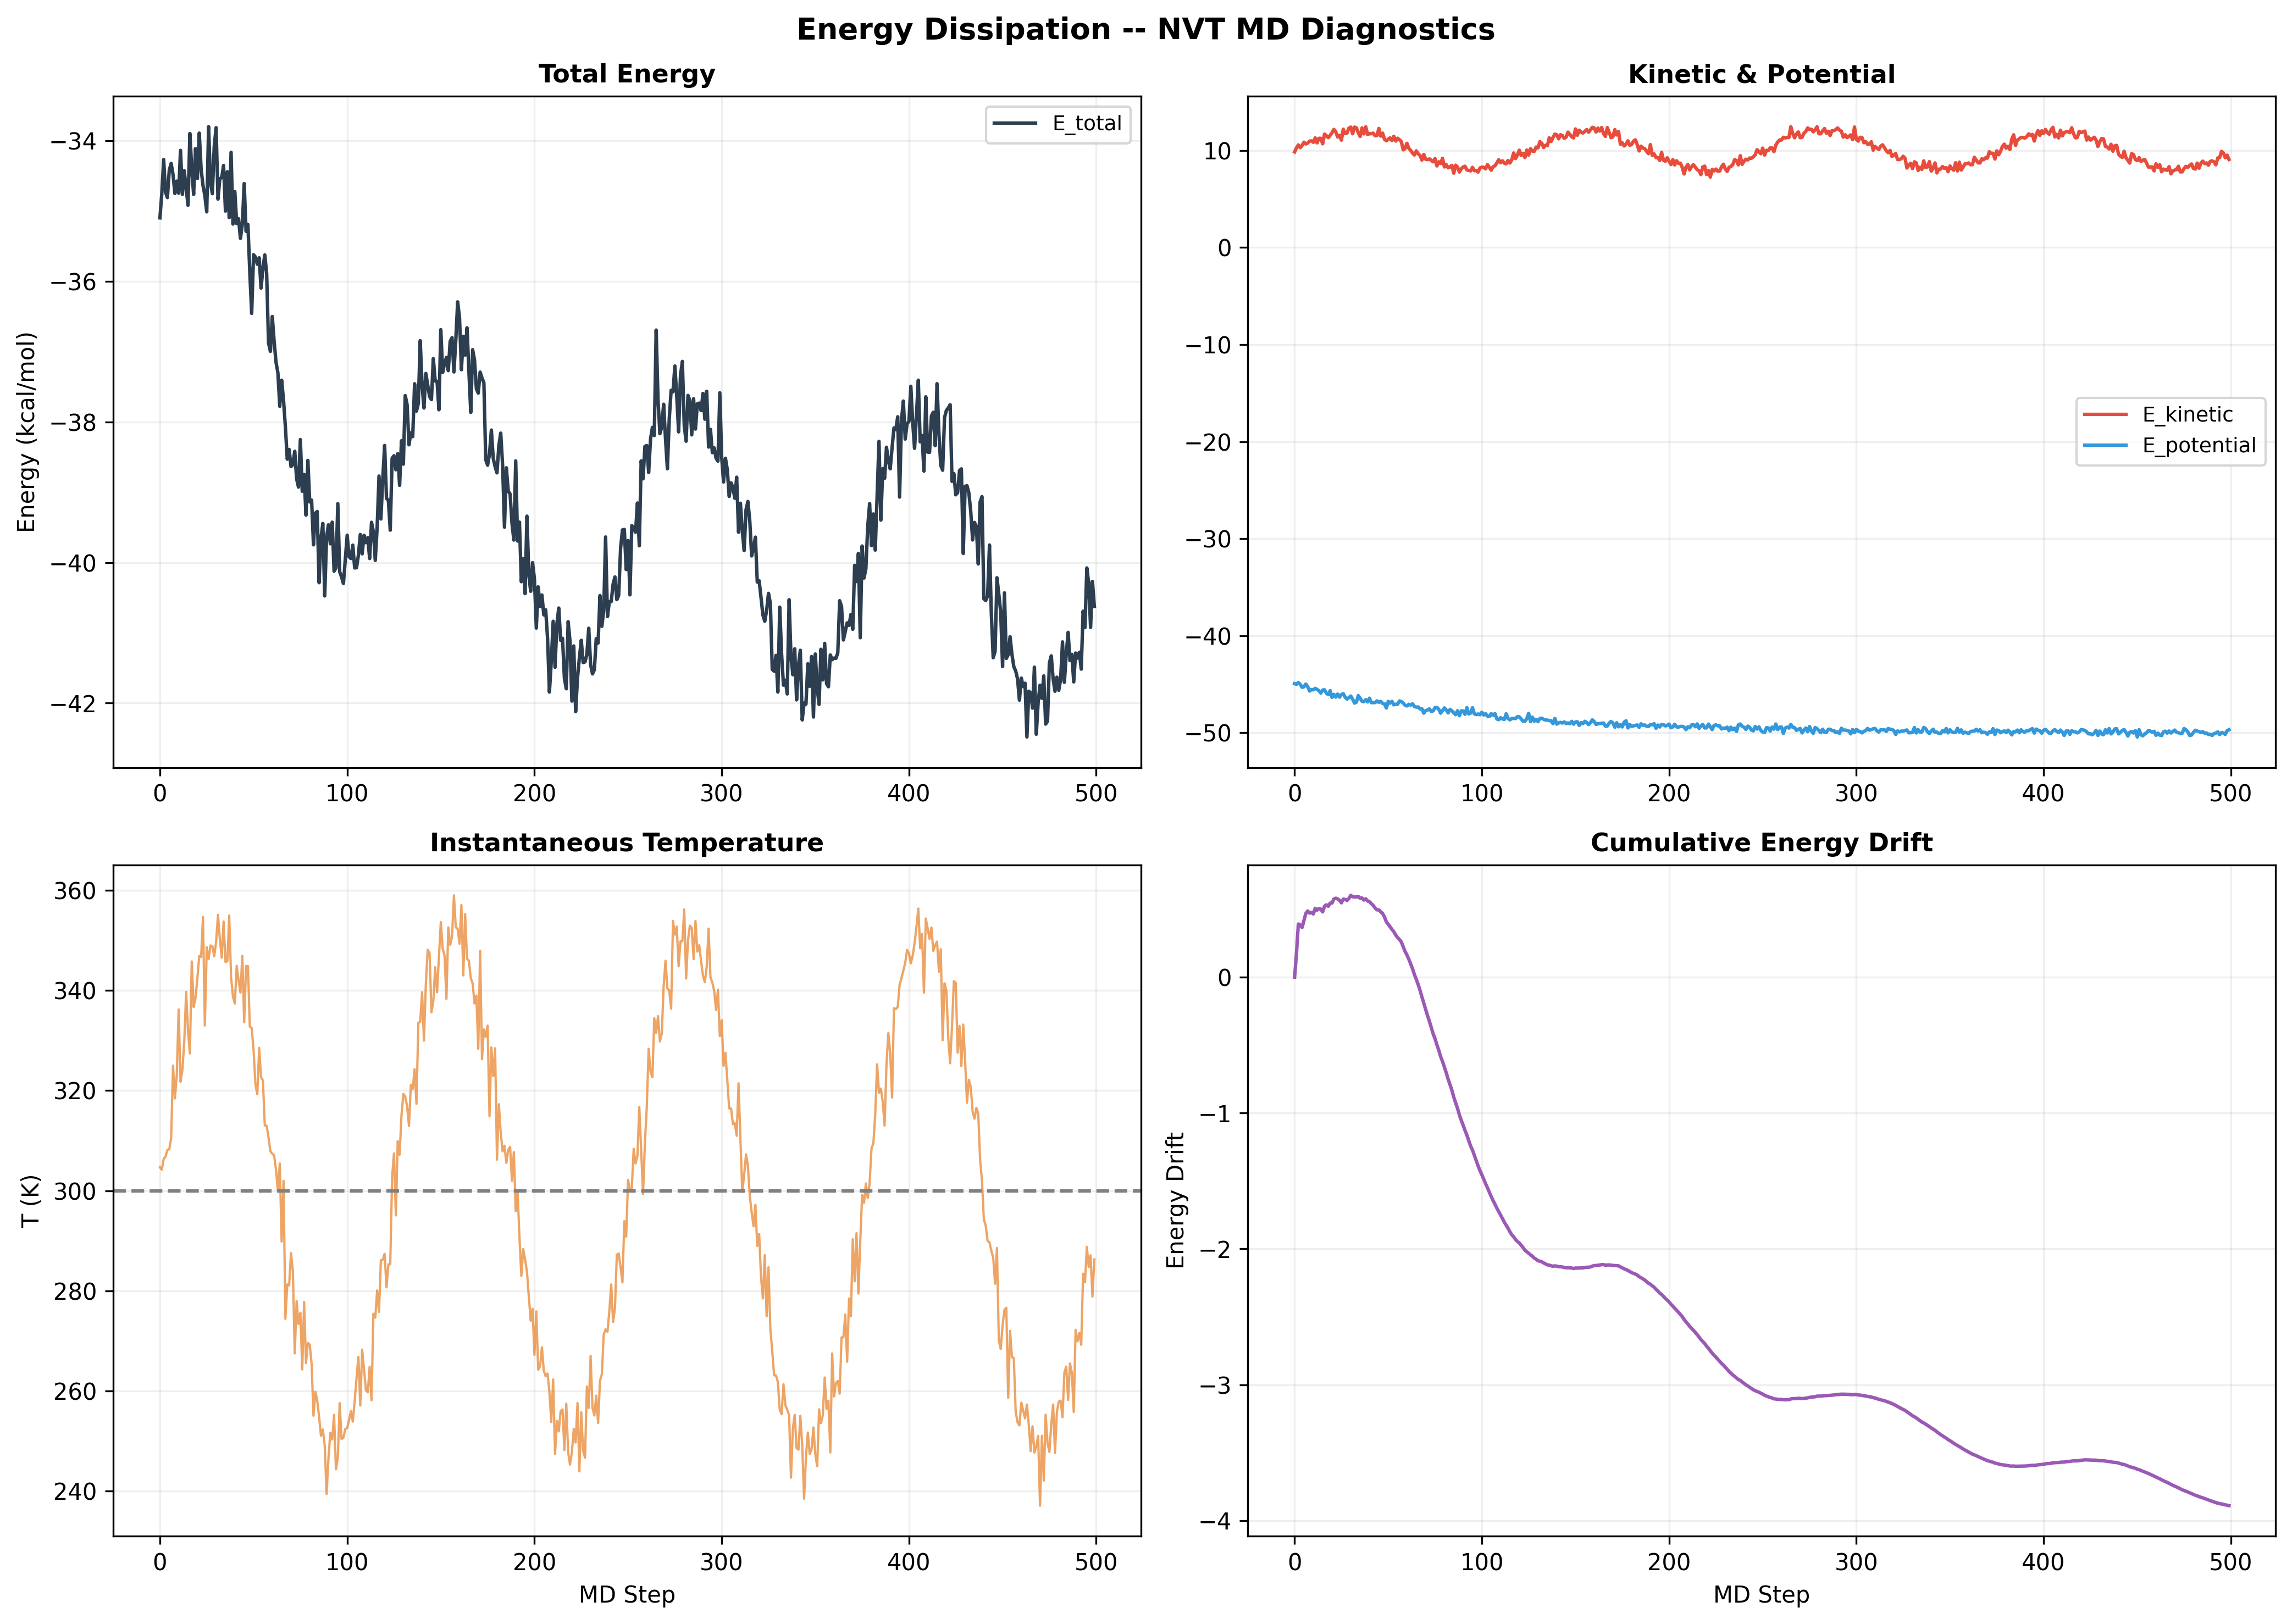
\includegraphics[width=\textwidth]{energy_dissipation.png}
\caption{Energy dissipation}
\end{subfigure}
\hfill
\begin{subfigure}[b]{0.30\textwidth}
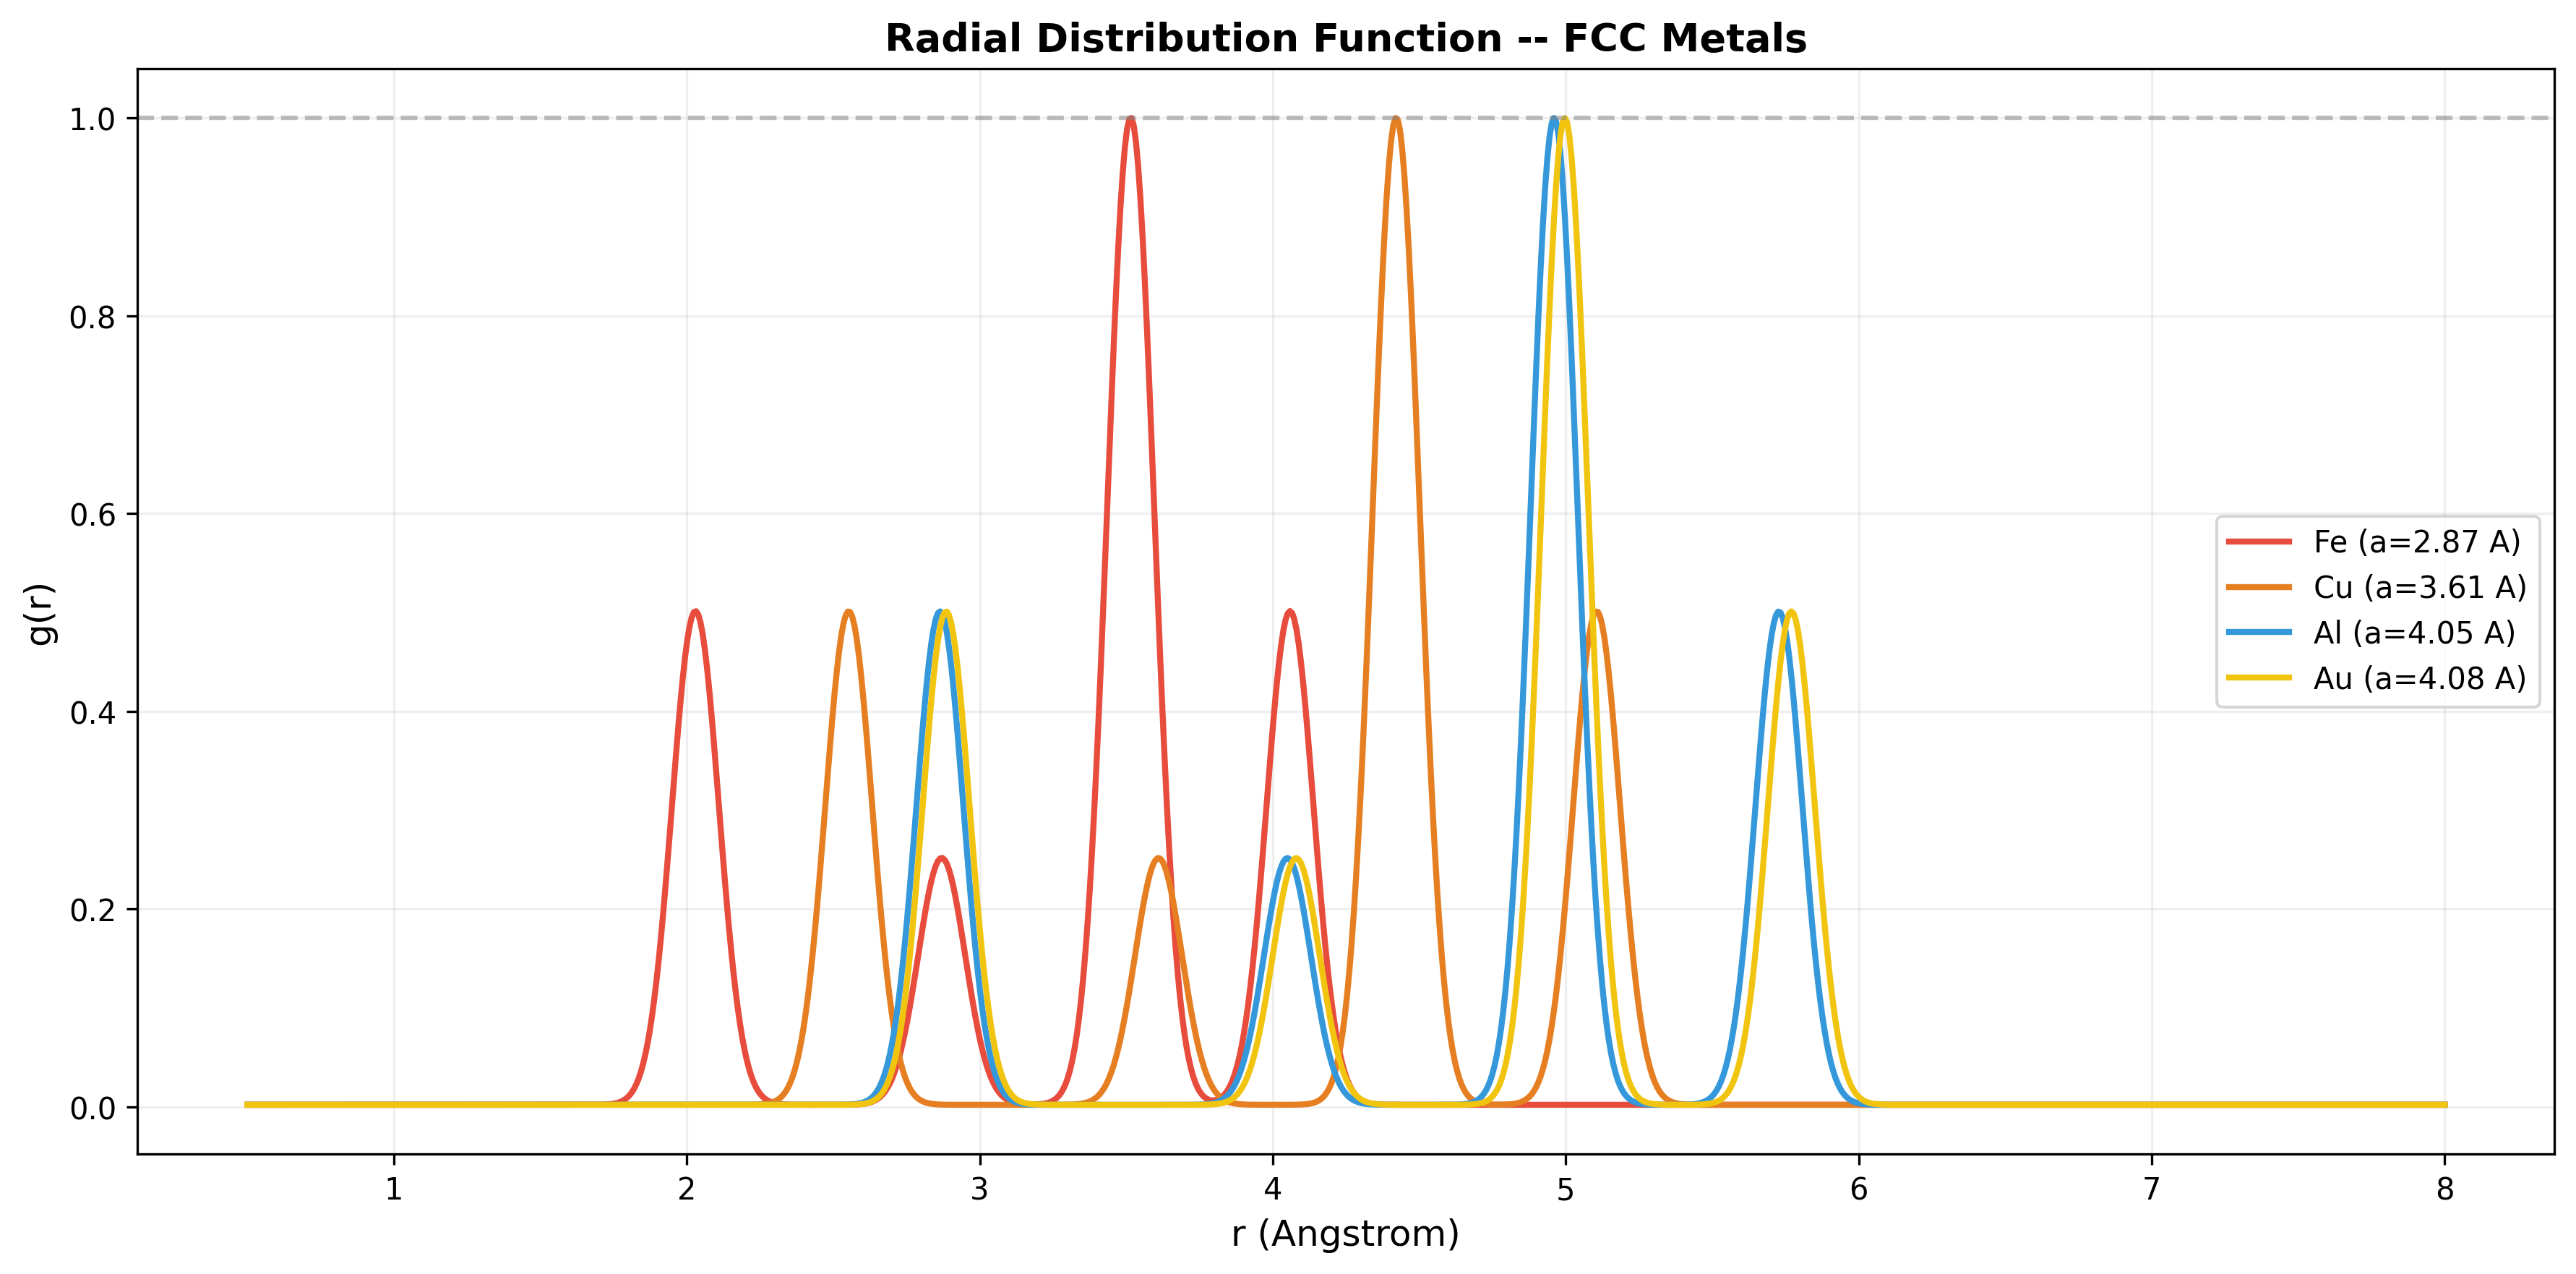
\includegraphics[width=\textwidth]{rdf_curves.png}
\caption{RDF curves}
\end{subfigure}
\hfill
\begin{subfigure}[b]{0.30\textwidth}
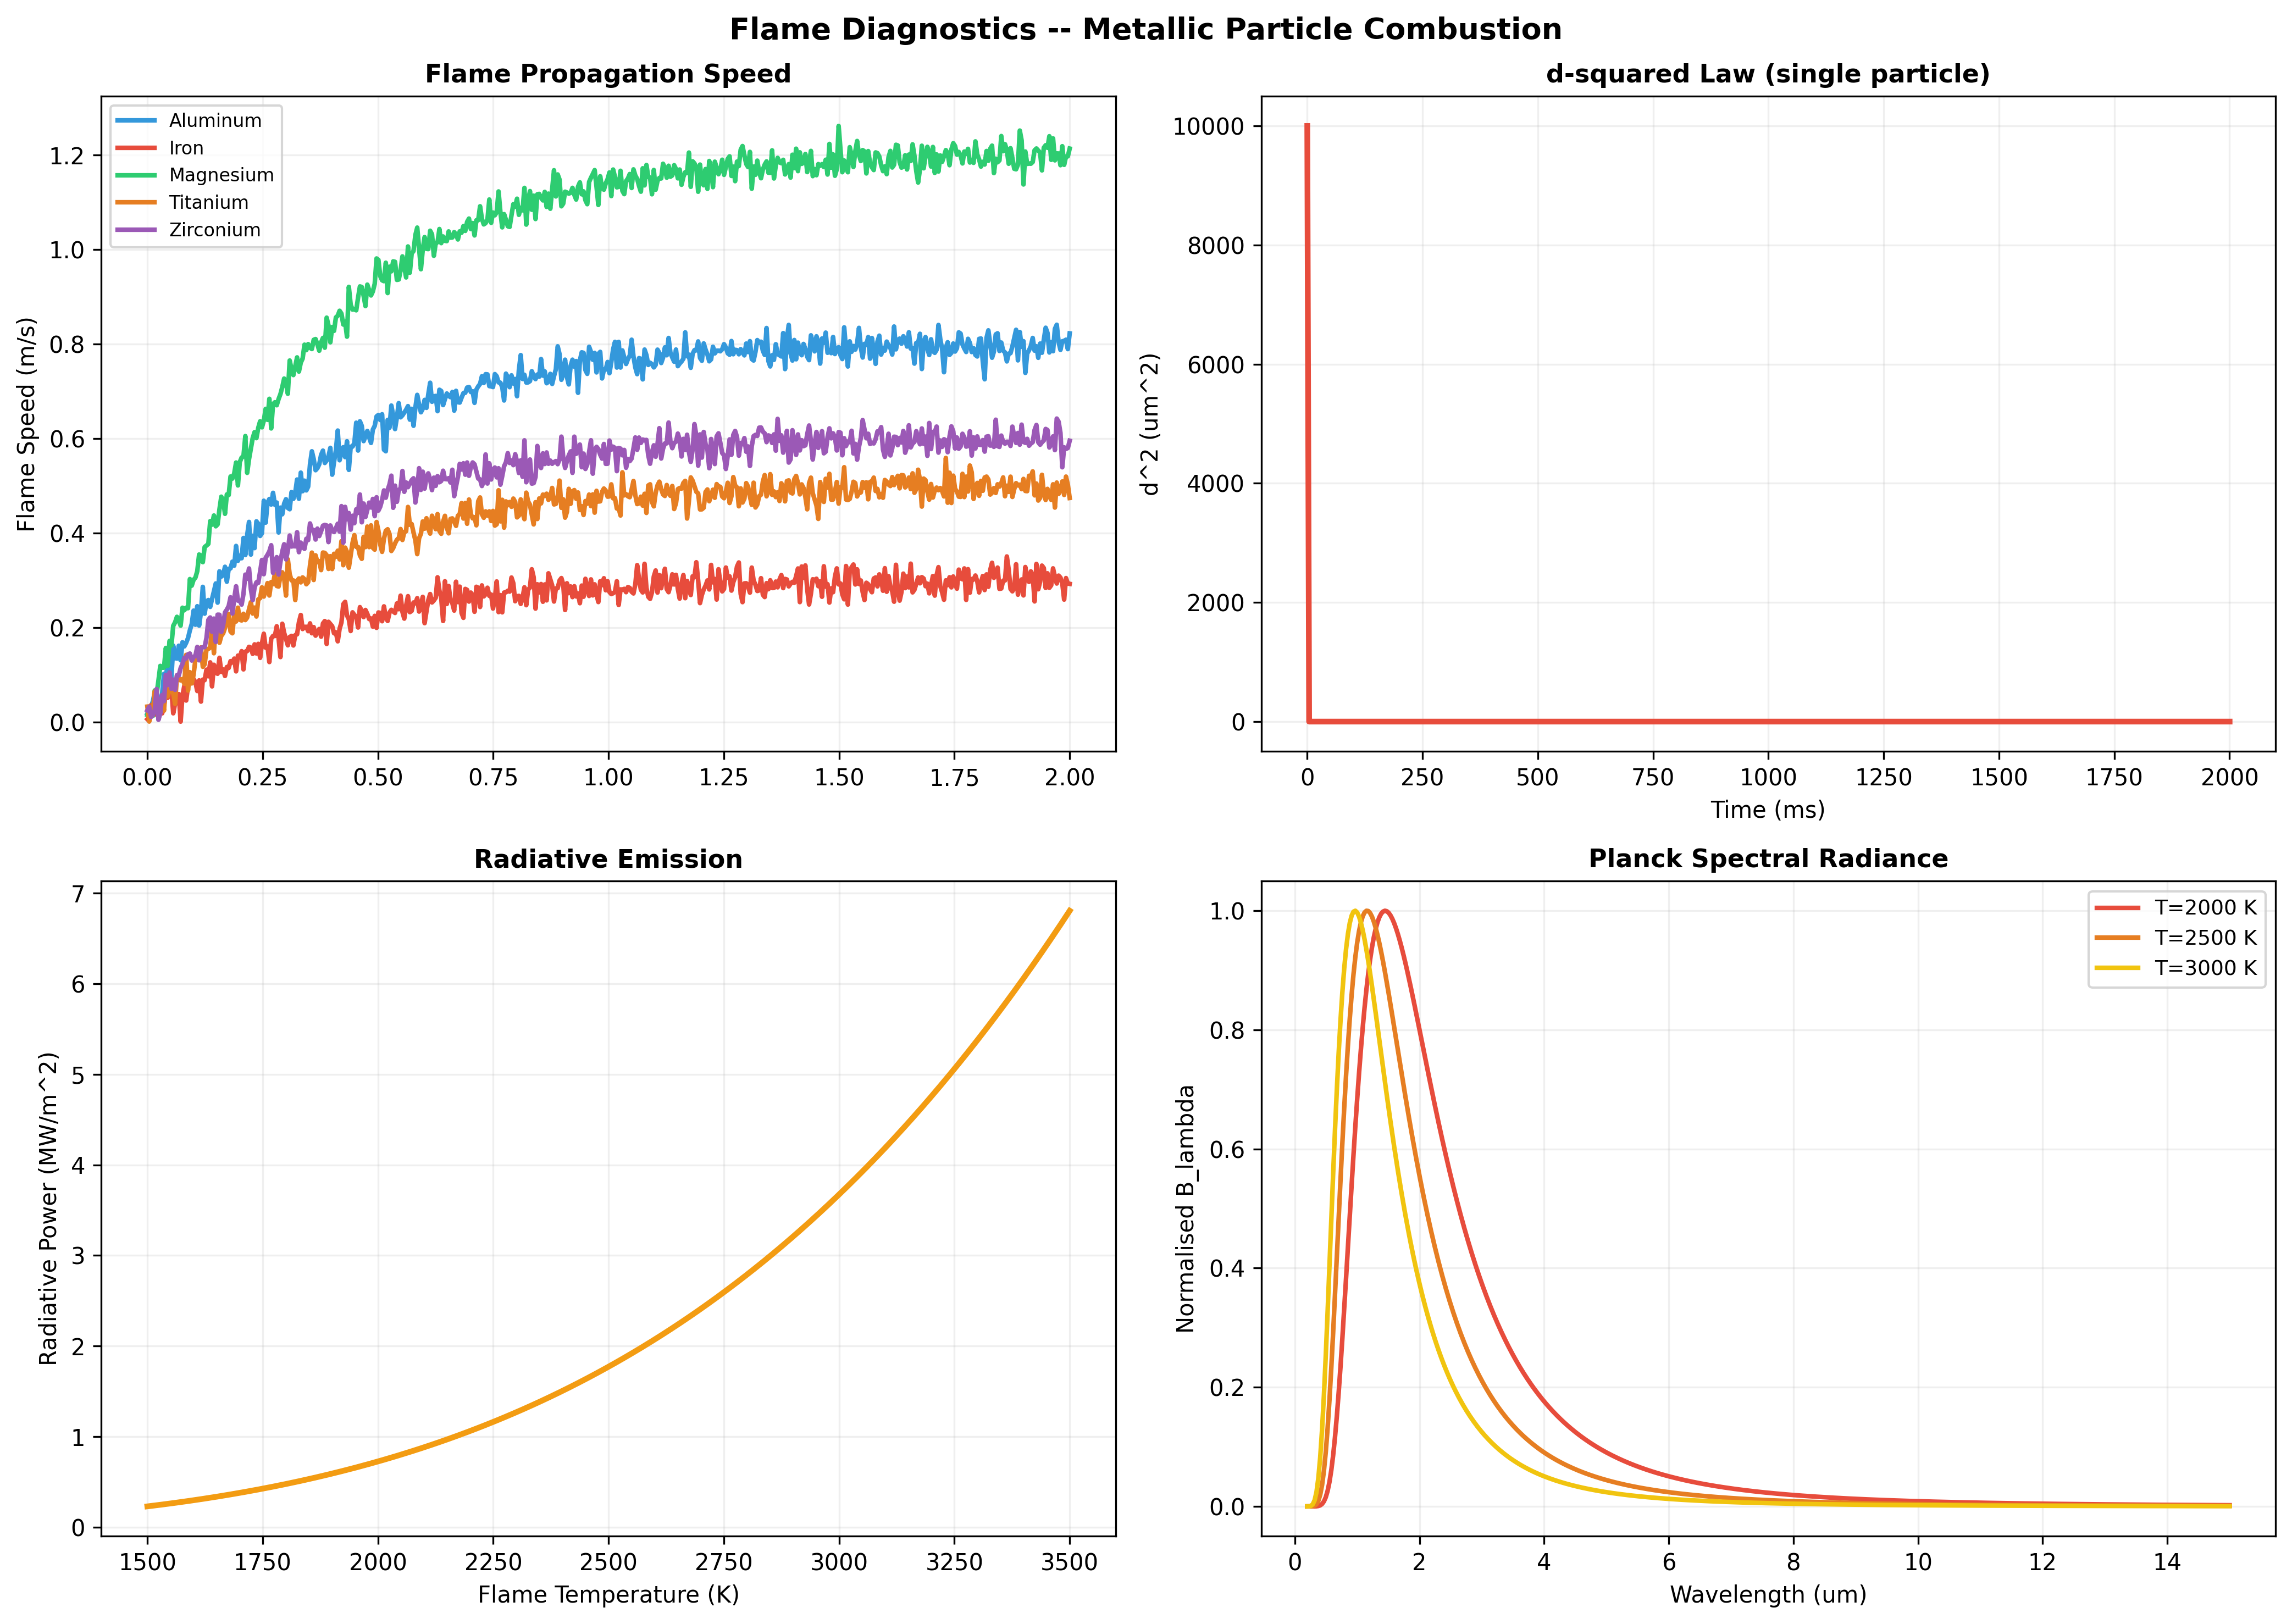
\includegraphics[width=\textwidth]{flame_dashboard.png}
\caption{Flame dashboard}
\end{subfigure}
\end{figure}

\begin{figure}[H]
\centering
\begin{subfigure}[b]{0.30\textwidth}
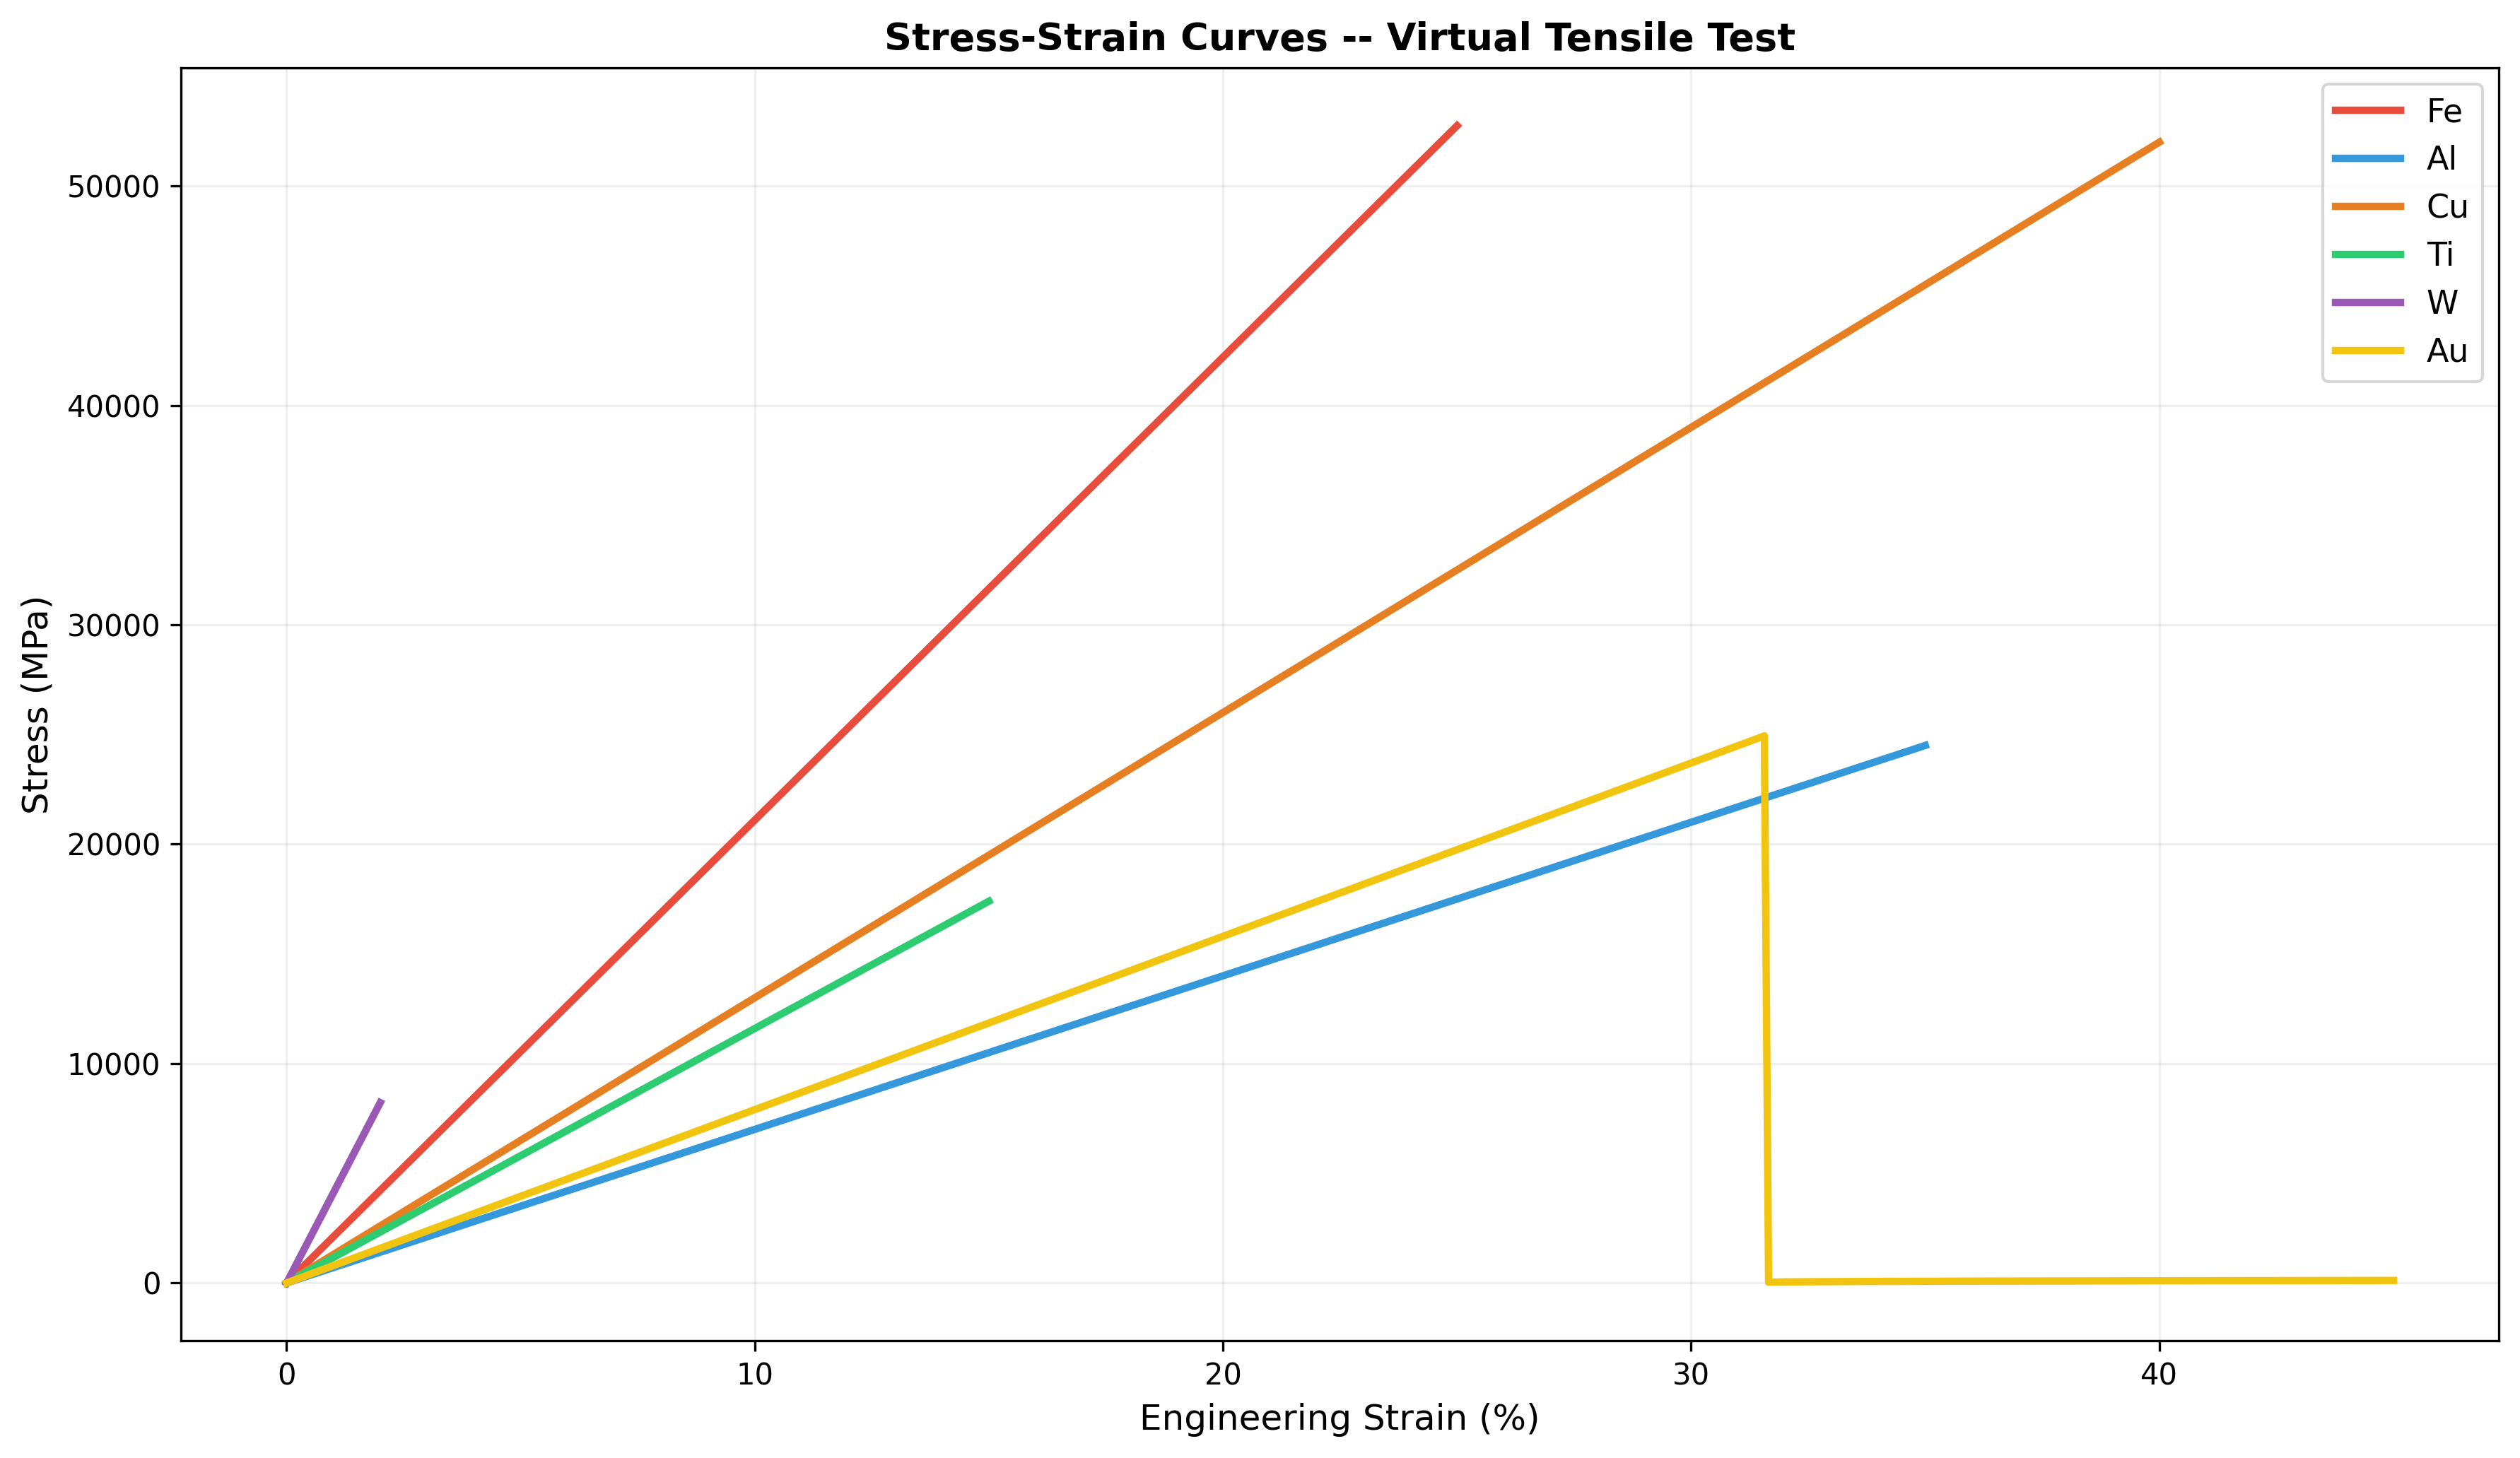
\includegraphics[width=\textwidth]{stress_strain.png}
\caption{Stress--strain}
\end{subfigure}
\hfill
\begin{subfigure}[b]{0.30\textwidth}
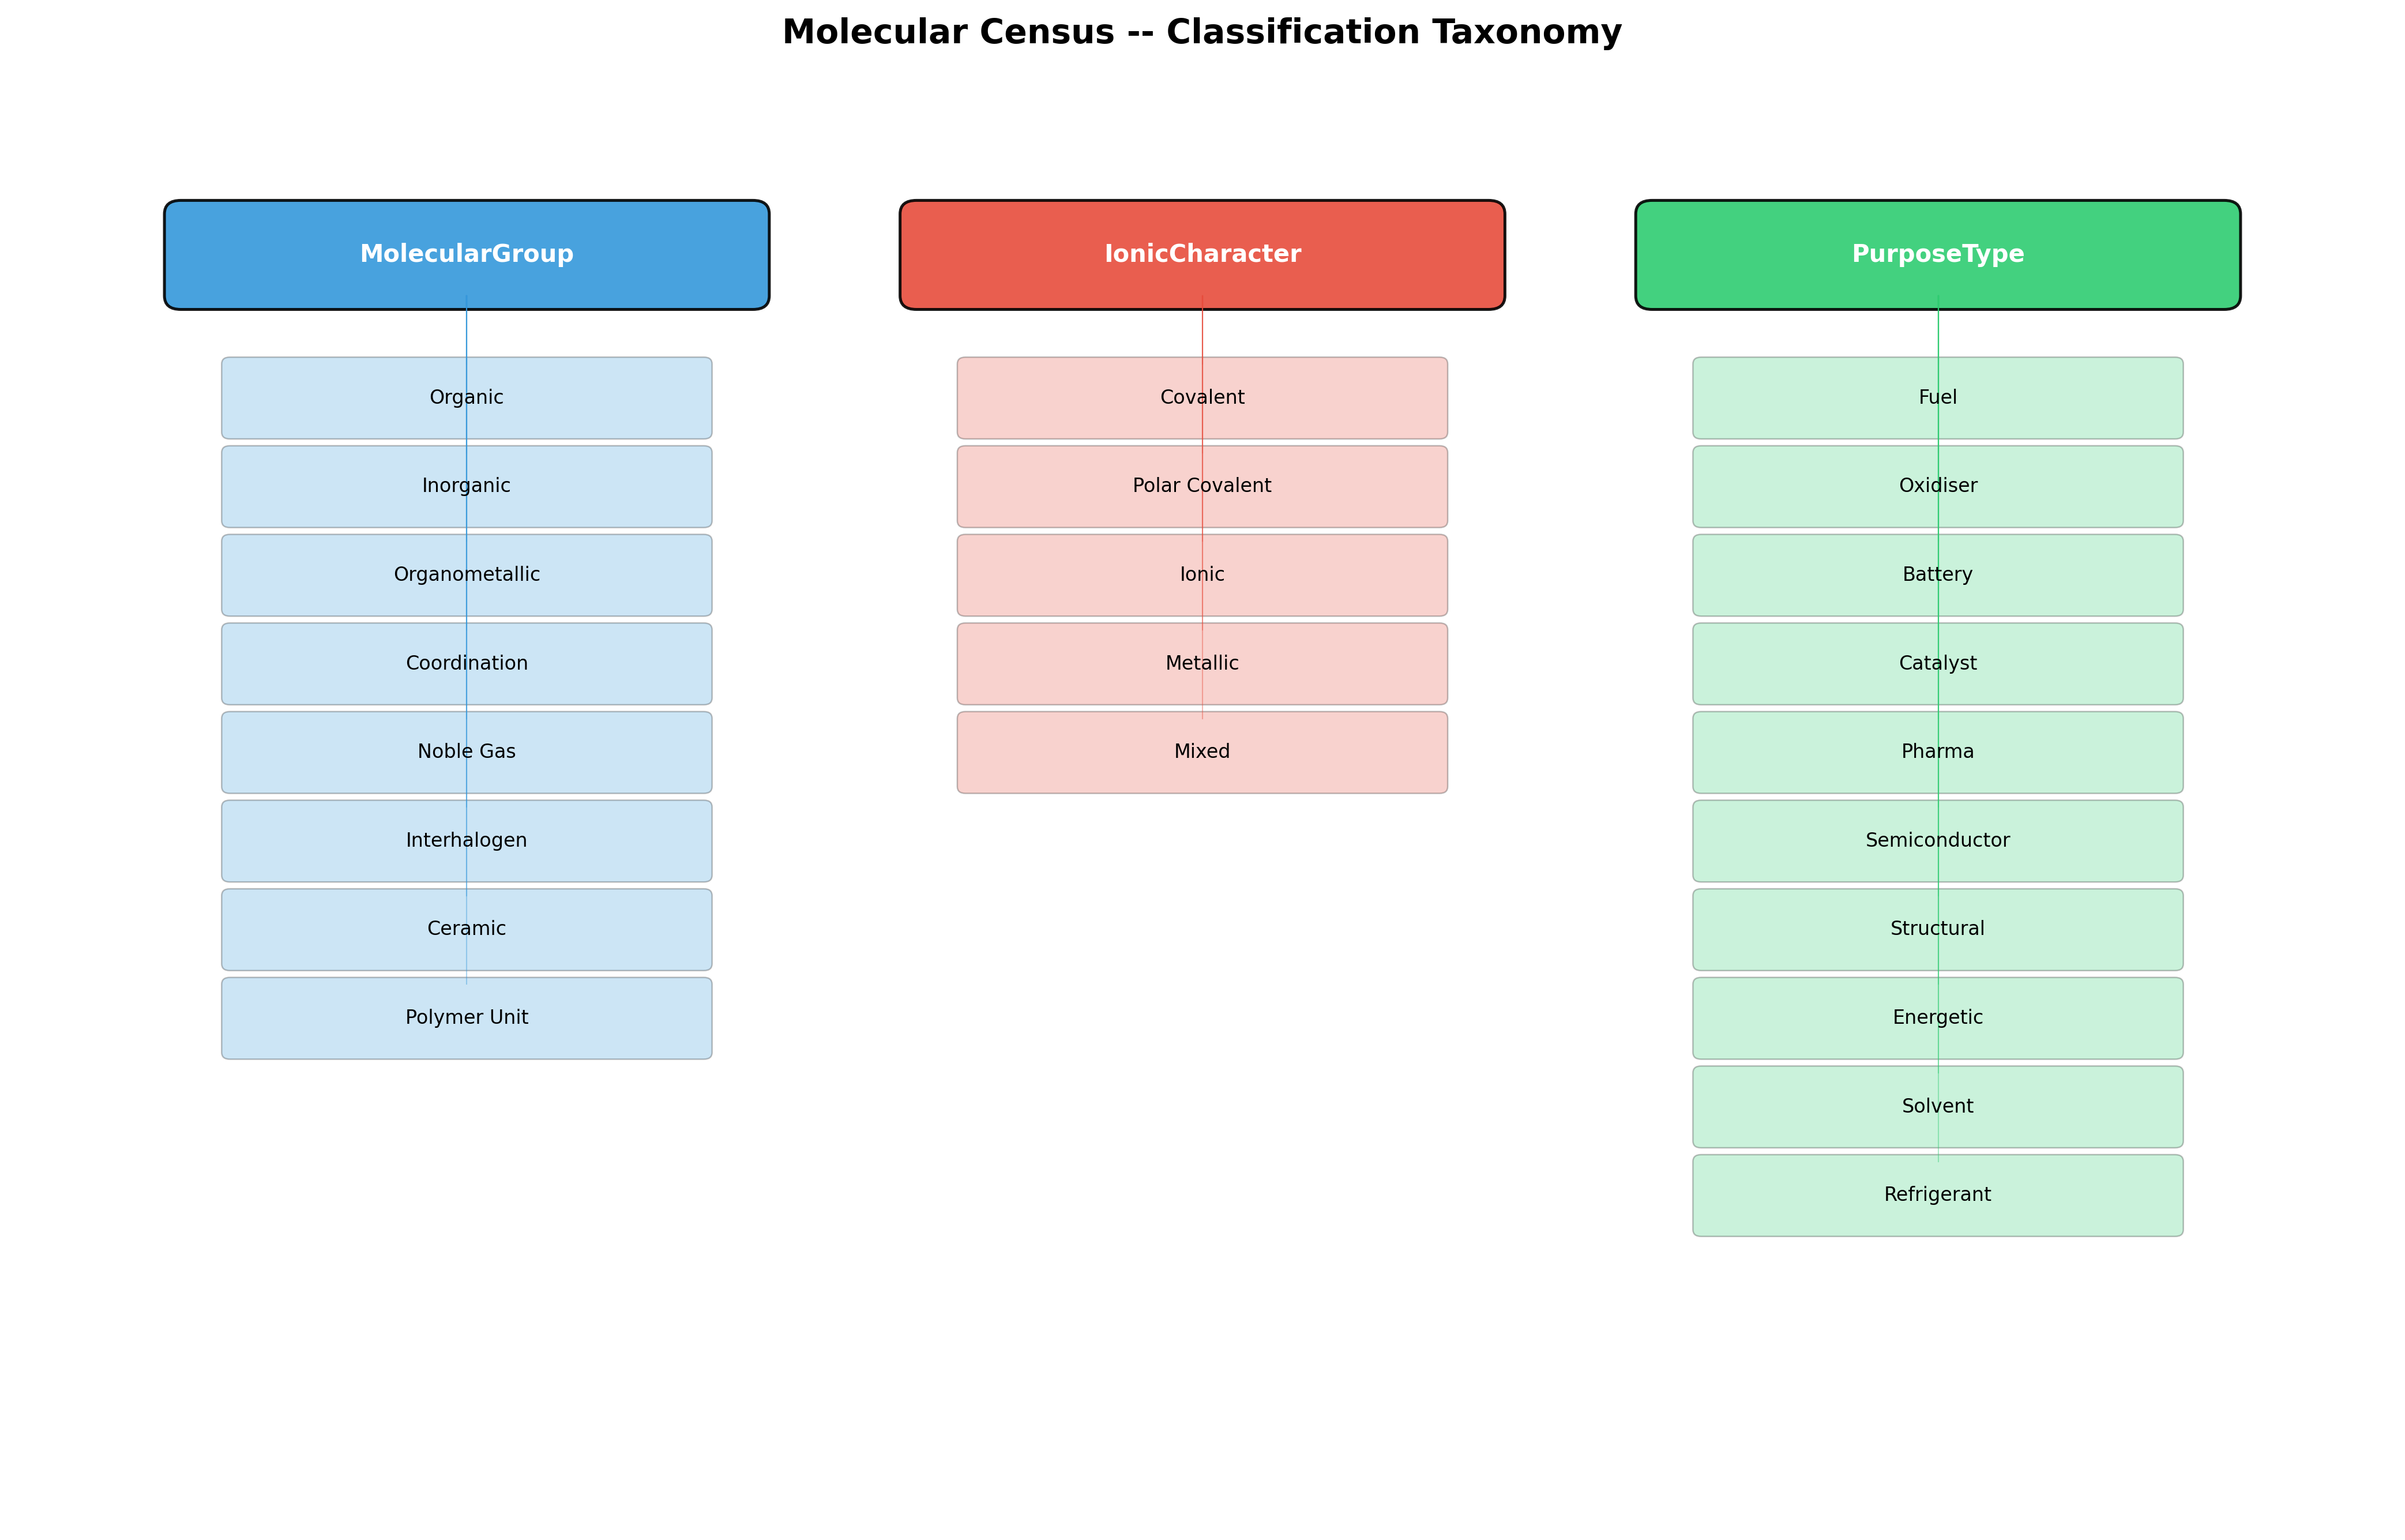
\includegraphics[width=\textwidth]{census_taxonomy.png}
\caption{Census taxonomy}
\end{subfigure}
\hfill
\begin{subfigure}[b]{0.30\textwidth}
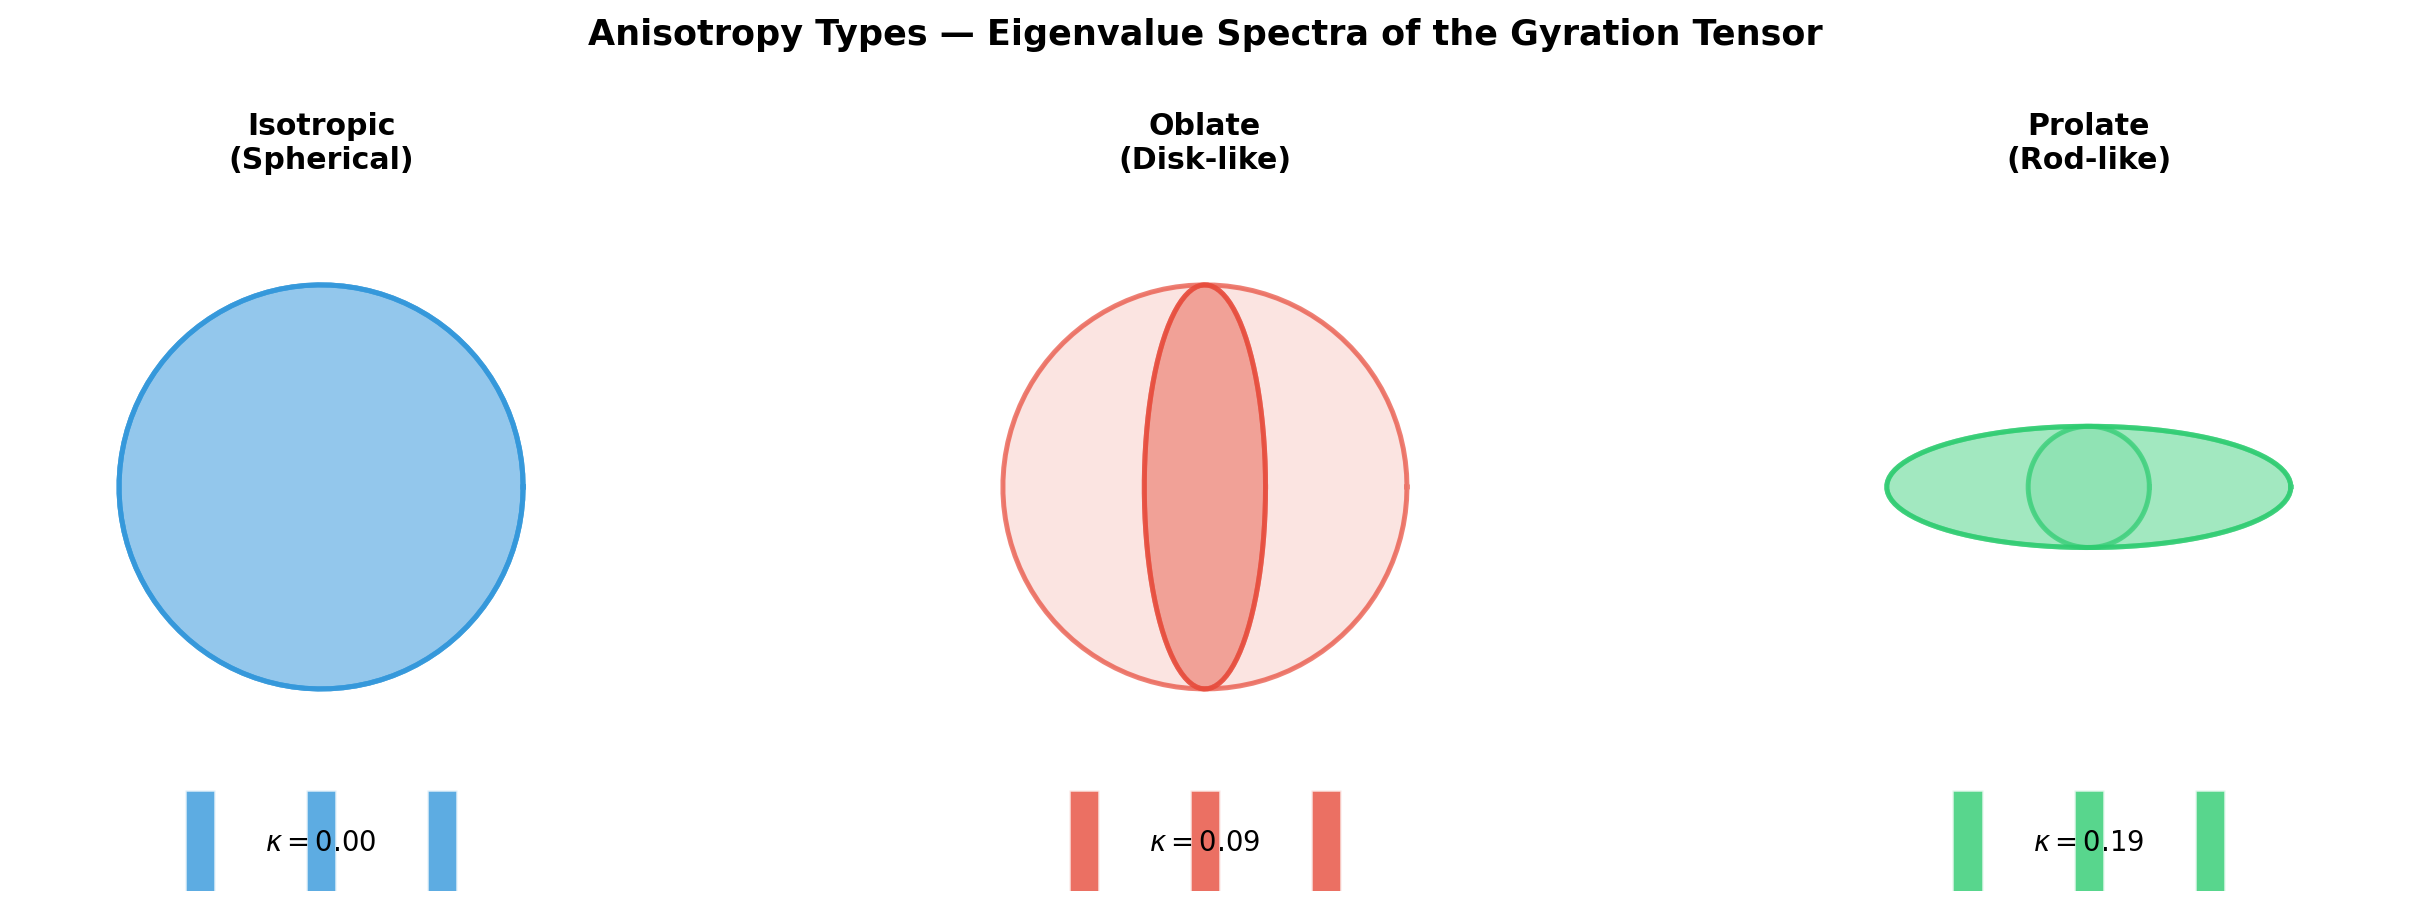
\includegraphics[width=\textwidth]{overview_anisotropy_types.png}
\caption{Anisotropy types}
\end{subfigure}
\end{figure}


% ════════════════════════════════════════════════════════════════════════════
\section{Build and Compilation Guide}
% ════════════════════════════════════════════════════════════════════════════

\subsection{C++ Build}
\begin{verbatim}
cmake -B build -G Ninja
cmake --build build
\end{verbatim}

\subsection{Test Execution}
\begin{verbatim}
cmake --build build --target test_state_c
./build/test_state_c          # 27 tests
cmake --build build --target test_emergence_dataset
./build/test_emergence_dataset # 25 tests
\end{verbatim}

\subsection{Figure Generation}
\begin{verbatim}
python scripts/render_document_figures.py   # 84 molecular figures
python scripts/render_overview_figures.py   # 12 overview figures
\end{verbatim}

\subsection{Documentation Compilation}
\begin{verbatim}
cd docs
# Individual documents:
pdflatex section1_foundational_thesis.tex

# Master compilation (744 pages):
pdflatex VSEPR_SIM_COMPLETE.tex
pdflatex VSEPR_SIM_COMPLETE.tex   # (second pass for TOC)
pdflatex VSEPR_SIM_COMPLETE.tex   # (third pass if needed)

# Quick index (this document):
pdflatex VSEPR_SIM_INDEX.tex
\end{verbatim}

\subsection{File Inventory Summary}

\begin{center}
\renewcommand{\arraystretch}{1.2}
\begin{tabular}{lr}
\toprule
\textbf{Category} & \textbf{Count} \\
\midrule
LaTeX source files     & 44 (42 sections + 2 master) \\
Compiled PDFs          & 44 \\
Total pages            & 744 (master) \\
Rendered PNG figures   & 96 \\
C++ headers            & 50+ \\
Test files             & 15 groups \\
Python scripts         & 5+ \\
\bottomrule
\end{tabular}
\end{center}


% ════════════════════════════════════════════════════════════════════════════
\section{Reading Paths}
% ════════════════════════════════════════════════════════════════════════════

\subsection{For Newcomers}
\begin{enumerate}
\item \textbf{METHODOLOGY\_2PAGE} --- 2-page executive summary
\item \textbf{section1\_foundational\_thesis} --- motivation and scope
\item \textbf{section2\_state\_ontology} --- core state definitions
\item \textbf{section\_visualization\_inspection} --- browse the figures
\item \textbf{section\_final\_statement} --- thesis conclusion
\end{enumerate}

\subsection{For Developers}
\begin{enumerate}
\item \textbf{section\_testing\_infrastructure} --- test framework
\item \textbf{section\_state\_c\_revised\_notation} --- current API ($S_0$/$S_f$)
\item \textbf{section\_layer\_stack} --- architecture overview
\item \textbf{section\_database\_architecture} --- data layer
\item \textbf{section\_bridge\_architecture} --- multi-scale coupling
\end{enumerate}

\subsection{For Researchers}
\begin{enumerate}
\item \textbf{section\_emergence\_dataset\_1} --- benchmark data schema
\item \textbf{deep\_research\_visual\_studies} --- research engine
\item \textbf{section\_organometallic\_folding\_adsorption} --- applied study
\item \textbf{section8\_9\_reaction\_electronic} --- reaction paths
\item \textbf{ehd\_theory} --- coupled EHD physics
\end{enumerate}

\subsection{Complete Volume}
Open \textbf{VSEPR\_SIM\_COMPLETE.pdf} (744 pages) for the full compilation
with all sections, overview figures, and five appendix figure galleries.

\end{document}
